%----------------------------------------------------------------------------------------
%	PACKAGES AND OTHER DOCUMENT CONFIGURATIONS
%----------------------------------------------------------------------------------------

	\documentclass[a4paper, 11pt, oneside]{book}

	\usepackage[sc]{mathpazo} % Use the Palatino font
	\usepackage[utf8]{inputenc}
	\usepackage[spanish, es-tabla]{babel}
	\decimalpoint
	
	\usepackage{lipsum}
	\usepackage{graphicx}
	\usepackage[T1]{fontenc} % Use 8-bit encoding that has 256 glyphs
	\linespread{1.15} % Line spacing - Palatino needs more space between lines
	%\usepackage{microtype} % Slightly tweak font spacing for aesthetics
	%
	\usepackage[hmarginratio=1:1,left=20mm, top=22mm]{geometry} % Document margins
	%\usepackage{multicol} % Used for the two-column layout of the document
	\usepackage[hang, small,labelfont=bf,up,textfont=it,up]{caption} % Custom captions under/above floats in tables or figures
	\usepackage{mathtools}
	%\usepackage{booktabs} % Horizontal rules in tables
	\usepackage{float} % Required for tables and figures in the multi-column environment - they need to be placed in specific locations with the [H] (e.g. \begin{table}[H])
	\usepackage{hyperref} % For hyperlinks in the PDF
	\usepackage{appendix}
	\usepackage{subcaption}
	%\usepackage{wrapfig}
	%%\usepackage[]{mcode} % For embebing matlab code
	%\usepackage[makeroom]{cancel}
	%
	%%\usepackage{lettrine} % The lettrine is the first enlarged letter at the beginning of the text
	%\usepackage{paralist} % Used for the compactitem environment which makes bullet points with less space between them
	%
	%\usepackage{abstract} % Allows abstract customization
	%\renewcommand{\abstractnamefont}{\normalfont\bfseries} % Set the "Abstract" text to bold
	%\renewcommand{\abstracttextfont}{\normalfont\small\itshape} % Set the abstract itself to small italic text
	%%%
	%\usepackage{titlesec} % Allows customization of titles
	%%\renewcommand\thesection{\Roman{section}} % Roman numerals for the sections
	%%\renewcommand\thesubsection{\Roman{subsection}} % Roman numerals for subsections
	%\titleformat{\section}[block]{\large\scshape\centering}{\thesection.}{1em}{} % Change the look of the section titles
	%\titleformat{\subsection}[block]{\large\centering}{\thesubsection.}{1em}{} % Change the look of the section titles
	%
	%\usepackage{fancyhdr} % Headers and footers
	%\pagestyle{fancy} % All pages have headers and footers
	%\fancyhead{} % Blank out the default header
	%\fancyfoot{} % Blank out the default footer
	%\fancyhead[C]{Titulo Corto% based on TRACS 
	%\hspace{4pt} $\bullet$ \hspace{4pt} MES ANO } % Custom header text
	%\fancyfoot[RO,LE]{\thepage} % Custom footer text
	%
	\usepackage{cite}
	\usepackage{listings}
	\usepackage{color}

	\graphicspath{{../Graphics/}}
	%
	%\DeclareGraphicsExtensions{.pdf,.png,.jpg} % Graphics type

	\newcommand{\gs}{encendido por ganancia}
	\newcommand{\ibias}{I_{bias}}
	\newcommand{\chirp}{$\nu_{chirp}$}
	\newcommand{\I}{corriente de inyecci\'on $I(t)$}
	\newcommand{\n}{$N(t)$}
	\newcommand{\s}{$S(t)$}
	\newcommand{\fase}{fase \'optica $\Phi(t)$}
%----------------------------------------------------------------------------------------
%	   METADATA
%----------------------------------------------------------------------------------------

	%\title{
	%	\selectfont\textbf{TITULO}% Article title
	%}

	%\author{
	%	\textsc{Jaime Diez Gonzalez-Pardo}\\
	%	%\thanks{A thank you or further information}\\ % Your name
	%	\fontsize{28pt}{10pt} Universidad de Cantabria \\ % Your institution
	%	%\thanks{A thank you or further information}\\[2mm] % Your name
	%	\normalsize gsdfgdfgdfgatura \\ 
	%	\normalsize{Compañeros:} \textsc{NOMBRE COMPANEROS }\\
	%	%\vspace{5mm}
	%}

	%\date{\today}
%----------------------------------------------------------------------------------------
%      · DOCUMENT
%----------------------------------------------------------------------------------------

	\begin{document}

		\begin{titlepage} 

			\newcommand{\HRule}{\rule{\linewidth}{0.5mm}} 
			
			\center % Centre everything on the page
			
			%------------------------------------------------
			%	Headings
			%------------------------------------------------
			
				%------------------------------------------------
				%	Logo
				%------------------------------------------------
				
					\begin{figure}[H]
						\centering
						\includegraphics[scale=0.6]{download.png}
					\end{figure}

					\textsc{\LARGE Facultad de Ciencias}\\[1.5cm] 
			
			
			%------------------------------------------------
			%	Title
			%------------------------------------------------
			
				\HRule\\[0.4cm]
				
				{\huge\bfseries Simulación de peines de frecuencia óptica generados por láseres de semiconductor}\\[0.8cm] % Title of your document

				{\huge Simulation of optical frequency comb generated by semiconductor lasers}\\[0.4cm] % Title of your document
				
				\HRule\\[1.5cm]

				{\Large Trabajo de Fin de Grado para acceder al}\\[0.4cm]

				{\LARGE\bfseries Grado en Física}\\[3cm]
			
			%------------------------------------------------
			%	Author(s)
			%------------------------------------------------
			
				\begin{flushright}
					\large
					\textit{Autor}\\
					Jaime \textsc{DÍEZ GONZÁLEZ-PARDO} \\ % Your name
					\large
					\textit{Director}\\
					Dr. Ángel \textsc{VALLE GUTIERREZ} % Supervisor's name
				\end{flushright}
			
			%------------------------------------------------
			%	Date
			%------------------------------------------------
			
				\vfill\vfill\vfill % Position the date 3/4 down the remaining page
				
				{\large\today} % Date, change the \today to a set date if you want to be precise
				
			%----------------------------------------------------------------------------------------
			
				\vfill % Push the date up 1/4 of the remaining page
		
		\end{titlepage}

			\begin{center}
				\textbf{ \large Agradecimientos}
			\end{center}
					
				Quiero dar las gracias a mi director de trabajo, el Prof. \'Angel Valle, no solo por toda la dedicaci\'on y apoyo mostrados en todo momento y por introducirme en el desconcocido mundo de la din\'amica no lineal, sino tambi\'en por animarme durante los \'ultimos d\'ias a realizar el \'ultimo gran esfuerzo, arrastr\'andole a \'el en ello.  \\
					
				Tambi\'en quiero dar las gracias a todas las personas que me han introducido en la f\'isica. En especial a mi profesor de m\'atematicas de secundaria, Feliz Horga, por aprovechar cualquier ocasi\'on para salirse del temario y enseñarnos las cosas tan bonitas que esconde la física, y a mi hermano Álvaro por transmitirme con tanta pasión todo lo que aprendia de física. \\

				Agradecerle a mi hermana, y en especial a mi padre, toda la paciencia que han demostrado tener estándo siempre ahi. Gracias tambiçén a toda la gente que me ha acompañado durante estos cuatro años, en especial a Inés que tantas horas me ha aguantado. \\

				Todo lo hago por tí, gracias Mamá.

			\newpage
			\begin{center}
				\textbf{\centering Resumen}
			\end{center}

				En este trabajo se han estudiado las caracteristicas de los peines de frecuencia \'optica en l\'aseres de semiconductor generados mediante las t\'ecnicas de \gs\ e inyecci\'on \'optica. Para ello se ha desarrollado un programa que ha permitido resolver las ecuaciones de balance mediante la implementaci\'on de un modelo num\'erico. Dichas ecuaciones de balance presentan t\'erminos de ruido estoc\'astico por lo que ha sido necesario utilizar m\'etodos de integraci\'on de ecuaciones diferenciales estoc\'asticas para su resoluci\'on.

				En la primera parte del trabajo se ha realizado el estudio de la simulación del l\'aser de semiconductor en solitario, analizando los resultados para el l\'aser en corriente cont\'inua y con \gs. Para el caso del l\'aser \gs\ se ha procedido a caracterizar los peines de frecuencia \'optica en funci\'on de la amplitud $V_{RF}$ y la frecuencia $f_R$ de la corriente inyectada. Se ha observado la creaci\'on y destrucci\'on de los peines a medida que se aumentaba la amplitud, as\'i como una mayor irregularidad para bajas frecuencias.

				En las siguientes partes se ha analizado la generaci\'on de peines de frecuencia \'optica mediante inyecci\'on de luz de un segundo l\'aser, caracterizada por la potencia inyectada $P_{Iny}$ y la diferencia de frecuencias entre ambos l\'aseres $\delta\nu$. Primero se ha estudiado el caso de inyecci\'on \'optica sin \gs, pasando a continuaci\'on a estudiar el caso de combinar ambos m\'etodos. El modelo ha permitido determinar las diferentes regiones dinámicas para distintas inyecciones, pudiendo identificar regiones con bifurcaciones de Hopf y de doblamiento de periodo.

				Se ha obtenido un excelente acuerdo entre los resultados de la simulación y los experimentales \cite{Chaves19}, mostrando la gran capacidad predictiva del modelo.
		
			\begin{center}
				\textbf{Palabras clave:} L\'aser de Semiconductor, Ecuaciones de Balance, Encendido por Ganancia, Inyecci\'on \'Optica, Peines de Frecuencia \'Optica.
			\end{center}

		\newpage
			\begin{center}
				\textbf{Abstract}
			\end{center}

				In this dissertation we have studied the characteristics of the optical frequency combs in semiconductor lasers generated by gain-switching and optical injection. A program has been developed to solve rate equations by implementing a numerical model. These rate equations present terms of stochastic noise, being necessary to use methods of integration of stochastic differential equations for their resolution. 
				
				In the first part of the work, the study of the simulation of the semiconductor laser alone has been carried out, analyzing the results for the laser in continuous wave and with gain-switching. In the case of the laser in gain-switching, the optical frequency combs have been characterized according to the amplitude $V_{RF}$ and the frequency $f_R$ of the injected current. The creation and destruction of combs has been observed as the amplitude was increased, as well as a greater irregularity for low frequencies.

				In the following parts the generation of optical frequency combs has been analyzed by means of optical injection from a second laser, characterized by the injected power $P_{Iny}$ and the detuning between both lasers' frequency $\delta\nu$. First, the case of optical injection without gain-switching has been studied, going on to study the combination of both methods. The model has allowed to determine the different dynamic regions for different injections, being able to identify regions with period doubling and Hopf bifurcations.

				An excellent agreement has been obtained between the simulation results and the experimental ones \cite{Chaves19}, showing the great predictive capacity of the model.

			\begin{center}
				\textbf{Key words:} Semiconductor Laser, Rate Equations, Gain Switching, Optical Injection, Optical Frequency Combs. 
			\end{center}

		%\thispagestyle{fancy} % All pages have headers and footers

		\tableofcontents

		%\listoffigures

		%----------------------------------------------------------------------------------------
		%	  ARTICLE CONTENTS
		%----------------------------------------------------------------------------------------

			\addtocontents{toc}{\vspace{0.01cm}}
			\chapter{Introducción} % Scope of the project = rad effects + minimization
				\label{Intr}

				\graphicspath{{../Graphics/Cpt1-Charactz/}}

\newcommand{\cw}{corriente continua}

Antes de abordar el estudio de la dinámica no lineal del láser de semiconductor de modo discreto se ha realizado la simulación del láser en solitario, sin inyección de luz del láser esclavo ($P_{Iny} = 0$). Se han realizado simulaciones para el láser tanto en \cw\ (CW de sus siglas en inglés), como en Gain-Switching, comparando los resultados con los obtenidos experimentalmente en condiciones similares \cite{Chaves19}.

	\addtocontents{toc}{\vspace{0.1cm}}
	\section{Láser en \cw}
		\label{Sol:CW}
		
		
Para poder realizar las simulaciones en \cw\ se ha trabajado con una corriente de inyección constante e igual a la corriente de polarización ($I(t) = I_{bias}$), tomando $V_{RF} = 0$.

HABLAR DE QUE EN CONTINUA SE TIENE QUE $\frac{\mathrm{d} N}{\mathrm{d} t} = \frac{\mathrm{d} S}{\mathrm{d} t} = \frac{\mathrm{d} \Phi}{\mathrm{d} t} = 0$

\addtocontents{toc}{\vspace{0.1cm}}
\subsection{Espectros de emisión}
	\label{Sol:CW:Spectr}

	Tal y como se vio en la sección \ref{Intr:LsrSmcdtr}, pequeñas variaciones en la corriente de inyección del láser producen desplazamientos de la línea de emisión del láser en el espectro de frecuencias. Por ello es importante conocer el valor de la longitud de onda del pico de emisión del láser en solitario en función de la corriente de polarización $\ibias$, de cara a realizar el estudio de la inyección de luz.

	En la Figura \ref{Img:spectrosCW} se muestran las densidades espectrales de potencia del láser a diferentes corrientes de polarización, comparando los datos obtenidos mediante la simulación del láser(Figura \ref{Img:spectrosCW:sim}), con los obtenidos experimentalmente(Figura \ref{Img:spectrosCW:exp}).

		% Img:spectrosCW {Img:spectrosCW:sim, Img:spectrosCW:exp}
		\begin{figure}[H]
			\centering
			\begin{subfigure}{0.45\textwidth}
				\centering
				\includegraphics[width=1.0\linewidth, height=6cm]{Espectros.png}
				\caption{\label{Img:spectrosCW:sim}Espectros ópticos obtenidos mediante simulación.}
			\end{subfigure}
			\begin{subfigure}{0.45\textwidth}
				\centering
				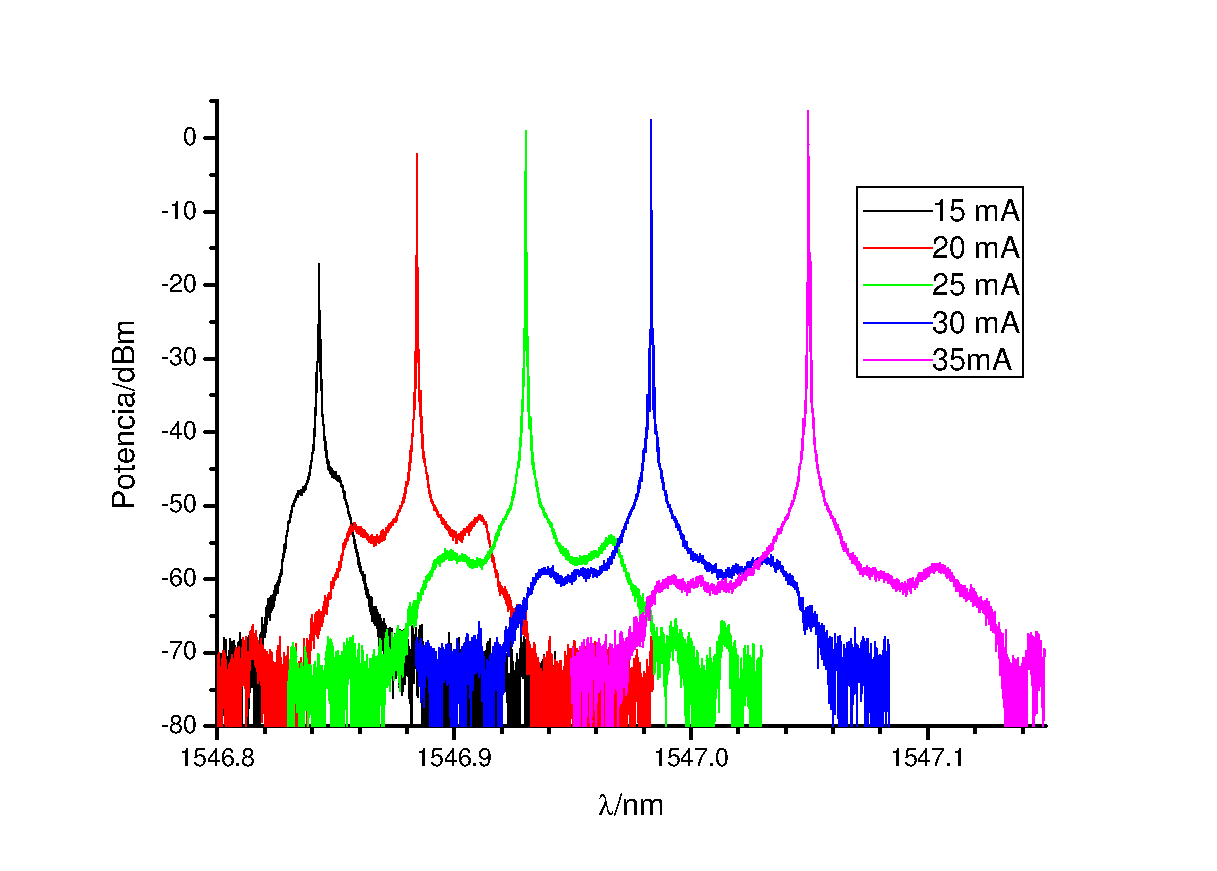
\includegraphics[width=1.0\linewidth, height=6cm]{../Chaves/OFC-GS/espectros_continua.png}
				\caption{\label{Img:spectrosCW:exp}Espectros ópticos obtenidos experimentalmente.}	
			\end{subfigure}
			\caption{\label{Img:spectrosCW}Espectros ópticos del DML para diferentes corrientes de polarización $\ibias$ obtenidos mediante simulación (izquierda \ref{Img:spectrosCW:sim}) y mediante experimento (derecha, \ref{Img:spectrosCW:exp}).}
		\end{figure}

		Comparando los espectros obtenidos mediante simulación con los obtenidos esperimentalmente se observa un gran parecido en la forma, observando una forma más puntiaguda y estrecha en los espectros con corriente $I_{bias}= 15$ mA para ambas gráficas. Además, la simulación permite observar los picos propios de las oscilaciones de relajación del láser que se observan en el experimento.

		Además, a partir de los espectros de la Figura \ref{Img:spectrosCW} se pueden obtener las longitudes de onda de los picos de emisión en función de la corriente $\ibias$. En la Tabla \ref{tab:lambdas} se muestran los valores de las longitudes de onda $lambda$ obtenidas de los espectros de la Figura \ref{Img:spectrosCW} tanto para la simulación como para el experimento.

		% tab:lambdas
		\begin{table}[H]
			\centering
			\begin{tabular}{c c c}
				\hline
				$\ibias$ & $\lambda_{sim}$ & $\lambda_{exp}$ \\\hline 
				15 & 1546.86 & 1546.84 \\
				20 & 1546.90 & 1546.88 \\
				25 & 1546.94 & 1546.93 \\
				30 & 1546.99 & 1546.98 \\
				35 & 1547.05 & 1547.05 \\\hline
			\end{tabular}
			\caption{\label{tab:lambdas}Longitud de onda de las lineas de emisión del DML en función de la $\ibias$ obtenidas de la figura \ref{Img:spectrosCW}. Se muestran los valores experimentales $\lambda_{exp}$ obtenidos de la gráfica \ref{Img:spectrosCW:exp} con un error de $\delta\lambda_{exp} = 0.02$, y los valores obtenidos de la simulación de la gráfica \ref{Img:spectrosCW:sim}.}
		\end{table}

	Los valores de las longitudes de onda que se muestran en la Tabla \ref{tab:lambdas} muestran una gran similitud entre los valores experimentales y los obtenidos mediante simulación, obteniendo una discrepancia máxima de $0.02$ nm. De esta forma, la gran concordancia entre los valores de $\lambda$ experimentales y los obtenidos a partir de la simulación, junto con la gran similitud en la forma de los espectros, muestra la capacidad de la simulación de reproducir computacionalmente los resultados obtenidos experimentalmente en el laboratorio.

	Para el estudio de la inyección de luz se trabajará con una corriente $I_{bias} = 35$ mA. Por tanto, la Tabla \ref{tab:lambdas} permite obtener su longitud de onda de emisión de $\lambda = 1547.05$ nm, siendo además la misma que la obtenida en el experimento.

\addtocontents{toc}{\vspace{0.1cm}}
\subsection{Oscilaciones de Relajación}
	\label{Sol:CW:RoF}

	Para que el láser comience a emitir se ha de cumplir que la emisión estimulada domine frente a la emisión espontánea. Esto se produce cuando la densidad de portadores de carga en la región activa supera un valor umbral, $N_{th}$, a partir del cuál el láser comienza a emitir fotones. Si la inyección de corriente que se le aplica al láser es constante (\cw), la densidad de portadores de carga tenderá a estabilizarse en $N_{th}$. De el mismo modo, la densidad de fotones y el chirp se estabilizarán para valores $S_{th}$ y $\Phi_{th}$.

	No obstante, si se parte de unas condiciones iniciales del láser con valores $N(t=0) < N_{th}$, será necesario que transcurra un cierto tiempo hasta que el láser alcance el equilibrio y se estabilice. A este tiempo se le denomina transitorio.

	Cabe destacar que, tal y como se comentó en el apartado \ref{Mdl:Code:Trans}, para la simulación se ha trabajado con un tiempo de transitorio $t_{trans} = 1.2$ ns, en el cuál se ha operado con la raiz cuadrada del módulo de $S$ en los términos de ruido para evitar resultados complejos, despeciando dicho intervalo en el estudio de los espectros. Sin embargo, en este apartado se estudiarán las ecuaciones de balance en el transitorio para corriente continua. El trabajar con una corriente continua mayor que la corriente umbral permite disminuir el intervalo de tiempo en el que se operará con $\sqrt{|S|}$ hasta los 0.2 ns, pudiendo realizar un estudio más riguroso de las ecuaciones de balance en el transitorio.

	Se considerará una intensidad de corriente $I(t)$ función escalón con $I(t>0) = \ibias$. En la ecuación \ref{eq:transient} se muestra la función escalón $I(t)$ utilizada así como las condiciones iniciales para la densidad de portadores de carga $N(0)$, la densidad de fotones $S(0)$ y de la fase óptica $\Phi(0)$.

		%eq:transient
		\begin{equation}
			\begin{matrix}
					I(t) = \left\{\begin{matrix}
									0 & t \leq 0\\ 
									\ibias = 30 \textrm{ mA} & t > 0
							\end{matrix}\right.
					& & & & & & 
					\begin{matrix}
						N(0) = N_{tr} \\ S(0) = 10^{15} \textrm{m}^{-3}\\ \Phi(0) = 0
					\end{matrix}
				\end{matrix}
			\label{eq:transient}
		\end{equation}

	En la Figura \ref{Img:transitorio} se muestra la evolución temporal de la \I\ junto con los valores obtenidos en la simulación para la \n\, la \s\ y la \fase\ para el transitorio $t_{trans} = 1.2$ ns.

		% Img:transitorio
		\begin{figure}[H]
			\centering
			\includegraphics[width=0.7\linewidth]{transitorio.png}
			\caption{\label{Img:transitorio}Evolución temporal de la \I, la \s, la \n\ y del \chirp\ durante el transitorio. Para la \I\ se ha marcado la corriente umbral del láser $I_{th} = 14.8$ mA con una línea horizontal discontinua.}	
		\end{figure}
		
		Se observan en las evoluciones temporales de \n, \s\ y \fase\ de la Figura \ref{Img:transitorio} tres regiones diferentes en función del comportamiento de las tres magnitudes: $i$) Una vez que la corriente inyectada supera la corriente umbral $I_{th}$ (en $t=0$) la \n\ comienza a aumentar. No obstante, el valor de $N(t)$ se mantiene inferior a $N_{th}$ por lo que no se produce emisión estimulada, y así, la densidad de fotones no aumenta y toma valores aleatorios, debido a la emisión espontánea, alrededor de $S(0)$. Esto también se puede observar en el comportamiento también aleatorio del \chirp. $ii$) La \n\ continua aumentando alcanzando el valor umbral $N_{th}$ en $t = 0.23$ ns. En este punto la densidad de fotones comienza a aumentar debido a la emisión estimulada producida al superar $N_{th}$. Sin embargo, al encontrarse $S(t)$ por debajo de $S_{th}$, $N(t)$ continua creciendo tomando valores por encima $N_{th}$ hasta que $S(t)$ alcanza el valor de $S_{th}$, en $t \approx 0.37$ ns. Al alcanzar $S(t)$ el valor de $S_{th}$, comienza a dominar la emisión estimulada frente a la emisión espontánea. Al alcanzar el valor $S_{th}$ la emisión estimulada domina frente a la emisión espontánea, como se puede observar el \chirp, y la densidad de portadores de carga comienza a disminuir, alcanzando la \n\ y \chirp\ un máximo. La densidad de fotones continúa aumentando y la densidad de portadores de carga disminuyendo, llegando nuevamente a tomar valores por debajo de $N_{th}$. Debido a ésto $S(t)$ alcanza un máximo cuando $N(t) = N_{th}$ y comienza a disminuir, volviendo a tomar valores inferiores a $S_{th}$ y así, volviendo a aumentar $N(t)$. Estas oscilaciones entorno a los valores umbrales continuan, disminuyendo su amplitud, realizando un comportamiento anarmónico y se las conoce como oscilaciones de relajación. En la figura \ref{Img:transitorio} se observan claramente estas oscilaciones, siendo iguales en el tiempo para \n\ y para el \chirp\ (máximos en el mismo tiempo $t$). También se observa la relación entre las oscilaciones de estas magnitudes con las de $S(t)$, obteniendo un máximo en $S(t)$ cuando $N(t) = N_{th}$ de tal forma que ambas oscilaciones tengan el mismo periodo. $ii$) Las oscilaciones de relajación van disminuyendo a medida que el tiempo avanza alcanzando el equilibrio en el que las tres magnitudes se mantienen constante.

		A partir de los datos de la figura \ref{Img:transitorio} se pueden obtener las frecuencias de las oscilaciones de relajación en el transitorio, a patir del tiempo entre los máximos. Una primera estimación permite obtener una frecuencia de oscilación de $\nu_{RoF} \approx 5.9$ GHz, que pasado a longitud de onda equivale a $\lambda = 0.05$ nm. Comparando dicho valor con los picos debidos a las oscilaciones de relajación de los espectros para $I = 30$ mA de la figura \ref{Img:spectrosCW} observamos que se encuentran en el mismo orden de magnitud, mostrando una gran concordancia entre la simulación y el experimento.


	\addtocontents{toc}{\vspace{0.1cm}}
	\section{OFC (Gain-Switching)}
		\label{Sol:OFC}

		
Para el estudio del m\'etodo de generaci\'on de OFC mediante \gs\ se ha trabajado con una corriente de inyecci\'on $I(t)$ modulada mediante una función sinusoidal superpuesta a una corriente de polarización $\ibias$ tal y como se muestra en la ecuación \ref{eq:gainSwtching}.

	\begin{equation}
		I(t) = \ibias + \frac{2\sqrt{2}V_{RF}}{Z_0+Z_l} \sin(2\pi f_R t)
		\label{eq:gainSwtching}
	\end{equation}

	Tal y como se vi\'o en el apartado \ref{Intr:OFC:GS} la calidad del \gs\ viene dada tanto por la intensidad de los picos como por la duraci\'on del pulso. De esta manera, se ha procedido a caracterizar los peines \'opticos de frecuencia en funci\'on del \gs\ aplicado modificando la frecuencia de oscilaci\'on y la amplitud de la corriente inyectada. Para el estudio del \gs\ en función de la frecuencia de oscilaci\'on se ha modificado el valor de $f_R$, estudiando primero los OFC para altas frecuencias ($f_R = 5.0$ GHz) y luego para bajas frecuencias ($f_R = 500$ MHz). Cabe destacar que al variar el valor de la frecuencia de oscilaci\'on $f_R$, la impedancia del l\'aser $Z_l$ tambi\'en cambia y as\'i también la suma $Z_0 + Z_l$.

	Para ambos valores de frecuencias $f_R$ se han estudiado los efectos producidos al variar la amplitud de la corriente de inyecci\'on, comparando tanto los espectros ópticos obtenidos como las variables dinámicas para diferentes amplitudes. Para el estudio con diferentes amplitudes ha bastado con modificar los valores de $V_{RF}$, ya que $(Z_0 + Z_l)$ solo varia para la frecuencia.

	\addtocontents{toc}{\vspace{0.1cm}}
	\subsection{Efecto de la amplitud de modulación a altas frecuencias}
		\label{Sol:OFC:HgFreq}

		Para el estudio del efecto de la amplitud de modulación a altas frecuencias se ha trabajado con una corriente de polarización $\ibias = 30$ mA y una frecuencia $f_R = 5.0$ GHz. Tal y como se vi\'o en el apartado \ref{Sol:CW:RoF}, la frecuencia de oscilaciones de relajación del l\'aser para $\ibias = 30$ mA es de $\nu_{RoF} \approx 5.9$ GHz, del orden de $f_R$. Se han resulto las ecuaciones de balance, obteniendo los OFC para tres amplitudes diferentes con $V_{RF}$: $0.05$ V, $1.00$ V y $1.50$ V. 

		En la Figura \ref{Img:rateEquations} se muestra la evolución temporal de la \I, la \s, la \n\ y de \chirp\ para varios valores de $V_{RF}$ pasada la zona del transitorio.

			% Img:rateEquations
			\begin{figure}[H]
				\centering
				\includegraphics[width=1.0\linewidth]{rateEquations.png}
				\caption{\label{Img:rateEquations}Evolución temporal de la \I ((a)-(c)), la \s ((d)-(f)), la \n\ ((g)-(i)) y del \chirp\ ((j)-(l)) en funci\'on de $V_{RF}$ pasada la zona del transitorio. Para la \I\ se ha marcado la corriente umbral del l\'aser $I_{th} = 14.8$ mA con una l\'inea horizontal discontinua. En la primera columna se muestran las evoluciones temporales para una amplitud de la corriente equivalente a $V_{RF} = 0.05$ V (verde), en la segunda columna para $V_{RF} = 1.00$ V (azul) y en la tercera columna de $V_{RF} = 1.50$ V(naraja).}	
			\end{figure}

		Mientras que para el caso del l\'aser en corriente continua ($I(t) = \ibias$) estudiado en la secci\'on anterior (secci\'on \ref{Sol:CW}), $S(t)$, $N(t)$ y el \chirp\ alcanzaban un valor constante pasado el transitorio, ahora la modulación en la corriente produce oscilaciones de igual periodo en $S(t)$, $N(t)$ y el \chirp. Se observa un aumento de la amplitud en $S(t)$, $N(t)$ y el \chirp\ al aumentar la amplitud de la corriente. Adem\'as, se observa como las oscilaciones en $N(t)$ y el \chirp\ van en fase (m\'aximos en el mismo tiempo $t$), mientras que los m\'aximos de $S(t)$ se obtienen cuando $N(t)$ decae a $N_{th}$.
			
		Para el caso de $V_{RF} = 0.05$ V, con una menor amplitud, se observa que las oscilaciones en la corriente (Figura \ref{Img:rateEquations} (a)) son pequeñas. Al igual que la corriente; la \s, la \n\ y el \chirp\ tambi\'en presentan oscilaciones de amplitud pequeña.% Cabe destacar que para este caso de amplitud pequeña, la \s\ (Figura \ref{Img:rateEquations} (d)) toma valores cercanos a cero, al no producirse ning\'un pico de intensidad. Esto produce que la emisi\'on estimulada no tome valores suficientemente altos como para que la emisi\'on espont\'anea sea despreciable y as\'i, se puede observar en el \chirp\ (Figura \ref{Img:rateEquations} (g)) el ruido debido a la emisión espont\'anea.

		Al aumentar la amplitud de la corriente a $V_{RF} = 1$ V (Figura \ref{Img:rateEquations} (b)) se observa como los aumentos de la corriente durante la oscilaci\'on coinciden con el crecimiento de \n\ (Figura \ref{Img:rateEquations} (k)), haciendo que tome valores muy superiores a $N_{th}$. A su vez, esto produce que, al superar $N(t)$ el valor del umbral $N_{th}$, la \s\ (Figura \ref{Img:rateEquations} (e)) tambi\'en tenga un pico superior al valor del l\'aser en corriente continua. De igual forma que ocurria en el transitorio, al aumentar $S(t)$ y dominar la emisi\'on estimulada, $N(t)$ comienza a disminuir, alcanzando un m\'aximo. Sin embargo, en el momento en el que $N(t)$ alcanza el m\'inimo, la corriente se encuentra por debajo de la corriente umbral $I_{th}$, y $N(t)$ no puede aumentar hasta que $I(t)$ toma nuevamente valores mayores de $I_{th}$. Debido a este tiempo $t$ en el que $N(t)$ no es capaz de volver a aumentar, compensando la disminuci\'on de \s, hay un mayor tiempo $t$ en el que $S(t)$ es cero, y as\'i no hay emisi\'on estimulada. Esta alternancia entre el dominio de la emisi\'on estimulada y la emisi\'on espont\'anea se puede pareciar en el \chirp\ (Figura \ref{Img:rateEquations} (h)), en la que se aprecia el ruido debido a la emisión espont\'anea cuando la densidad de fotones es cero, mienstras que durante los picos de $S(t)$ el ruido es despreciable y no se observa.
			
		Para la amplitud de $V_{RF} = 1.5$ V se observa la misma tendencia que para $V_{RF} = 1$ V, a excepci\'on de que en este caso, al aumentar la amplitud aumenta el tiempo en el que la corriente es menor que $I_{th}$ y as\'i el tiempo en el que $S(t)$ es cero y domina la emisi\'on espontánea.


		En la Figura \ref{Img:PSD} se muestran los espectros de los OFC obtenidos mediante \gs\ para las tres amplitudes de la Figura \ref{Img:rateEquations}.

			% Img:PSD
			\begin{figure}[H]
				\centering
				\includegraphics[width=1.0\linewidth]{PSD.png}
				\caption{\label{Img:PSD}Espectros de los OFC obtenidos mediante \gs\ para $\ibias = 30$ mA, $f_R = 5$ GHz y amplitud de modulaci\'on $V_{RF} = 0.05$ V (verde), $1.00$ V (azul) y $1.50$ V (naranja).}
			\end{figure}
			
		Al igual que se obtuvo en la Figura \ref{Img:rateEquations}, se puede observar como el caso de la amplitud de modulaci\'on $V_{RF} = 0.05$ V se asemeja al del l\'aser en corriente cont\'inua, obteniendo un espectro (Figura \ref{Img:PSD} (verde)) con la frecuencia de emisi\'on dominante de la Figura \ref{Img:spectrosCW}. Como consecuencia del \gs\ realizado se observan excitadas las frecuencias de emisi\'on, apareciendo nuebas l\'ineas de emisi\'on a los lados de la emisi\'on principal.

		Para el caso de $V_{RF} = 1$ V se observa un OFC (Figura \ref{Img:PSD} (azul)) de gran calidad formado por numerosas l\'ineas de emisión equiespaciadas y bien definidas. Se ha obtenido una regi\'on de longitudes de onda con l\'ineas de emisión de la misma densidad espectral de potencia lo cuál resulta enuna gran calidad del OFC.

		Por otro lado, se observa que para el caso de $V_{RF} = 1.5$ V (Figura \ref{Img:PSD} (naranja)) el OFC se detruye debido al ruido de la emisión espont\'anea, obteniendo l\'ineas de emisión poco definidas, con un espaciado variado y mucho ruido.

		De esta forma, se ha podido caracterizar la calidad de los OFC, y del \gs, para altas frecuencias en función de la amplitud de modulaci\'on. Se ha podido observar la creaci\'on del OFC para $V_{RF} = 1$ V, as\'i como la destrucci\'on de este para altas amplitudes, con $V_{RF} = 1.5$ V.

		Tal y como se ha comentado a partir de los resultados de la Figura \ref{Img:rateEquations}, uno de los efectos de aumentar la amplitud de modulaci\'on es la disminuci\'on de la corriente por debajo de $I_{th}$ por un tiempo $t$, que aumenta con la amplitud. Sin embargo, \'esto también se puede controlar para una amplitud fija, variando la corriente de polarizaci\'on $\ibias$.

		En la Figura \ref{Img:current} se muestran la potencia $P(t)$, obtenida a partir de la \s\ \ref{eq:Power}, y los espectros de los OFC con $f_R = 5$ GHz, $V_{RF} = 1$ V e $\ibias = 30$ mA y $50$ mA.

			% Img:current
			\begin{figure}[H]
				\centering
				\includegraphics[width=1.0\linewidth]{current.png}
				\caption{\label{Img:current}Perfil temporal de las potencias $P(t)$ (izquierda) y espectros (derecha) de OFC con $f_R = 5$ GHz, $V_{RF} = 1$ V e $\ibias = 30$ mA (azul) y $50$ mA (naranja).}	
			\end{figure}

		En el perfil temporal de la potencia $P(t)$ de $\ibias = 30$ mA (Figura \ref{Img:current} (izquierda, azul)) se observan las zonas de tiempo con $P(t) \propto S(t) = 0$ vistas en la Figura \ref{Img:rateEquations}, debidas a que la corriente toma valores por debajo de $I_{th}$ y as\'i \n\ no puede aumentar. De igual manera se ha obtenido un OFC de gran calidad (Figura \ref{Img:current} (derecha, azul)) como el obtenido en la Figura \ref{Img:PSD}.

		Sin embargo, en el caso de $\ibias = 50$ mA, al aumentar la corriente de polarizaci\'on, \'esta desplaza la función sinusoidal de la intensidad alejandola de $I_{th}$ y as\'i la amplitud de modulaci\'on no es suficiente para llegar a cruzar $I_{th}$. Esto se puede observar en que el perfil temporal de $P(t)$ (Figura \ref{Img:current} (izquierda, naranja)) no toma nunca el valor cero y as\'i realiza oscilaciones completas. Puesto que la frecuencia $f_R$ y la amplitud $V_{RF}$ de modulación s\'i son suficientes com para que se d\'e \gs, se observa un espectro (Figura \ref{Img:current} (derecha, naranja)) con un OFC formado por l\'ineas bien definidas e igualmente espaciadas. No obstante, el OFC obtenido para $\ibias = 50$ mA es m\'as estrecho que el obtenido para $\ibias = 30$ mA, careciendo de una meseta bien definida con l\'ineas de emisi\'on con densidad espectral de potencia similar. Debido a esto, el OFC obtenido para $\ibias = 30$ mA es de mayor calidad que el obtenido para $\ibias = 50$ mA.

		Otro de los efectos de aumentar la $\ibias$ de tal manera que no cruce la $I_{th}$ es la falta de una regi\'on donde domine la emisi\'on espont\'anea, como ocurria en la Figura \ref{Img:rateEquations}. Esto se puede observar en el menor ruido obtenido en el espectro para $\ibias = 50$ mA (Figura \ref{Img:current} (derecha, naranja)) frente al obtenido en el espectro de $\ibias = 30$ mA (Figura \ref{Img:current} (derecha, azul)).

	\addtocontents{toc}{\vspace{0.1cm}}
	\subsection{Efecto de la amplitud de modulación a bajas frecuencias}
		\label{Sol:OFC:LwFreq}

		Para el estudio del efecto de la amplitud de modulación a bajas frecuencias se ha trabajado con una corriente de polarización $\ibias = 50$ mA y una frecuencia $f_R = 500$ MHz. Se han obtenido la potencia $P(t)$ y los OFC para cuatro amplitudes diferentes, tomando cuatro valores distintos para $V_{RF}$: $0.05$ V, $0.4$ V, $1.0$ V y $1.2$ V.

		En la Figura \ref{Img:500} se muestran los perfiles temporales de la potencia $P(t)$ y los espectros de los OFC para $\ibias = 50$ mA, $f_R = 500$ MHz y $V_{RF} = 0.05$ V, $0.4$ V, $1.0$ V y $1.2$ V.
			% Img:500
			\begin{figure}[H]
				\centering
				\includegraphics[width=1.0\linewidth]{500.png}
				\caption{\label{Img:500}Perfiles temporales de la potencia $P(t)$ (fila superior) y espectros (fila inferior) de los OFC para $\ibias = 50$ mA, $f_R = 500$ MHz y $V_{RF} = 0.05$ V (primera columna), $0.4$ V (segunda columna), $1.0$ V (tercera columna) y $1.2$ V (cuarta columna).}	
			\end{figure}

		Al igual que se obtuvo en el apartado anterior para el caso de altas frecuencias con $\ibias = 50$ mA (Figura \ref{Img:current}), se observan en la Figura \ref{Img:500} perfiles temporales de la potencia oscilantes entorno al valor de la potencia en corriente continua ($P_{CW} \approx 4.7$ mW), variando su amplitud en funci\'on de la amplitud de modulación. Al tener una $\ibias$ muy superior a $I_{th}$ y una frecuencia baja, la amplitud de modulaci\'on no permite mantener la corriente de inyecci\'on por debajo de la corriente umbral un tiempo suficiente como para que $P(t) \propto S(t) = 0$, tal y como se observa en las Figuras \ref{Img:500} (fila superior).

		Para el caso de la amplitud de modulaci\'on pequeña con $V_{RF} = 0.05$ V, se ha obtenido un comportamiento muy similar a la corriente continua, al igual que para altas frecuencias. El espectro obtenido para esta amplitud de modulaci\'on es similar al de la Figura \ref{Img:PSD} (verde) del apartado anterior, obteniendo un pico de emisi\'on dominante correpondiente a la emisi\'on en continua y dos picos a cada lado debidos a la excitaci\'on de la frecuencia de oscilación.

		Se observa como, al igual que ocurria en a altas frecuencias, a medida que aumenta la amplitud de modulación aumenta el n\'umero de l\'ineas de emisión de espectro, llegando a destruirse para altas amplitudes de modulación. Sin embargo, al trabajar a bajar frecuencias se observa una clara irregularidad en el perfil del OFC, tomando los picos valores muy diversos de la densidad espectral de potencia. Esto implica una perdida de la calidad de los OFC a bajas frecuencias con respecto a altas frecuencias. 

		DEBERIA HABLAR SOBRE LOS PICOS QUE SE OBSERVAN EN LA POTENCIA PARA V = 1.2

		En la Figura \ref{Img:500mhz} se muestran los perfiles temporales de la potencia $P(t)$ y los espectros de los OFC para $\ibias = 50$ mA, $f_R = 500$ MHz y $V_{RF} = 0.1$ V, $0.4$ V, $1.2$ V y $1.6$ V obtenidos experimentalmente \cite{Chaves19}.

			% Img:500mhz
			\begin{figure}[H]
				\centering
				\includegraphics[width=1.0\linewidth]{../Chaves/OFC-GS/500mhz.png}
				\caption{\label{Img:500mhz}Perfiles temporales de la potencia $P(t)$ (fila superior) y espectros (fila inferior) de los OFC para $\ibias = 50$ mA, $f_R = 500$ MHz y $V_{RF} = 0.1$ V (primera columna), $0.4$ V (segunda columna), $1.2$ V (tercera columna) y $1.6$ V (cuarta columna) obtenidos experimentalmente \cite{Chaves19}.}	
			\end{figure}

		En la Figura \ref{Img:500mhz} se muestran la potencia $P(t)$ y los espectros experimentales para diferentes amplitudes de modulación, permitiendo comparar los resultados obtenidos mediante simulación con los obtenidos en el laboratorio.

		En la cuarta columna de la Figura \ref{Img:500mhz} se muestran los resultados obtenidos para una amplitud de $V_{RF} = 1.6$ V, observando como el espectro de frecuencia se encuentra completamente destruido. Dichos resultados no pudieron ser obtenidos mediante la simulación debido al problema en el transitorio con $\sqrt{S(t)}$. En la primera columna de la Figura \ref{Img:500mhz} se muestran los resultados para una amplitud de modulación pequeña de $V_{RF} = 0.1$ V. Al igual que en los resultados de la simulación, se obtiene un comportamiento similar al de la corriente continua con un pico de emisi\'on dominante. No obstante, al tratarse de el doble de la amplitud utilizada en la simulaci\'on de la Figura \ref{Img:500} se obtienen un mayor n\'umero de picos de emisión estimulados. Los resultados que se muestran en la segunda columna de la Figura \ref{Img:500mhz}  para $V_{RF} = 0.4$ V equivalen a los resultados de la simulación de la segunda columna de la Figura \ref{Img:500}. En ambas figuras se pueden observar un OFC con un perfil aproximandamente sim\'etico con un pico de menor intensidad en el centro. Por \'ultimo, la tercera columna de la Figura \ref{Img:500mhz} equivale a la cuarta columna de la Figura \ref{Img:500}. Ambos espectros presentan un perfil similar con un aumento brusco de la densidad espectral de potencia de los picos para bajas longitudes de onda, seguido de una disminuci\'on m\'as tenue para lontitudes de onda mayores. Ambos perfiles temporales de potencia presentan LOS PICOS DE LOS QUE HE DE HABLAR.

	El excelente acuerdo entre los resultados de la simulaci\'on de la Figura \ref{Img:500} y los resultados experimentales de la Figura \ref{Img:500mhz} indican la capacidad de la simulaci\'on de explicar los procesos que involucra el \gs\ en la generaci\'on de OFC, pudiendo servir para la caracterizaci\'on de la calidad de los OFC.



				
			\addtocontents{toc}{\vspace{0.01cm}}
			\chapter{Modelo Computacional}
				\label{Mdl}

				\graphicspath{{../Graphics/Cpt1-Charactz/}}

\newcommand{\cw}{corriente continua}

Antes de abordar el estudio de la dinámica no lineal del láser de semiconductor de modo discreto se ha realizado la simulación del láser en solitario, sin inyección de luz del láser esclavo ($P_{Iny} = 0$). Se han realizado simulaciones para el láser tanto en \cw\ (CW de sus siglas en inglés), como en Gain-Switching, comparando los resultados con los obtenidos experimentalmente en condiciones similares \cite{Chaves19}.

	\addtocontents{toc}{\vspace{0.1cm}}
	\section{Láser en \cw}
		\label{Sol:CW}
		
		
Para poder realizar las simulaciones en \cw\ se ha trabajado con una corriente de inyección constante e igual a la corriente de polarización ($I(t) = I_{bias}$), tomando $V_{RF} = 0$.

HABLAR DE QUE EN CONTINUA SE TIENE QUE $\frac{\mathrm{d} N}{\mathrm{d} t} = \frac{\mathrm{d} S}{\mathrm{d} t} = \frac{\mathrm{d} \Phi}{\mathrm{d} t} = 0$

\addtocontents{toc}{\vspace{0.1cm}}
\subsection{Espectros de emisión}
	\label{Sol:CW:Spectr}

	Tal y como se vio en la sección \ref{Intr:LsrSmcdtr}, pequeñas variaciones en la corriente de inyección del láser producen desplazamientos de la línea de emisión del láser en el espectro de frecuencias. Por ello es importante conocer el valor de la longitud de onda del pico de emisión del láser en solitario en función de la corriente de polarización $\ibias$, de cara a realizar el estudio de la inyección de luz.

	En la Figura \ref{Img:spectrosCW} se muestran las densidades espectrales de potencia del láser a diferentes corrientes de polarización, comparando los datos obtenidos mediante la simulación del láser(Figura \ref{Img:spectrosCW:sim}), con los obtenidos experimentalmente(Figura \ref{Img:spectrosCW:exp}).

		% Img:spectrosCW {Img:spectrosCW:sim, Img:spectrosCW:exp}
		\begin{figure}[H]
			\centering
			\begin{subfigure}{0.45\textwidth}
				\centering
				\includegraphics[width=1.0\linewidth, height=6cm]{Espectros.png}
				\caption{\label{Img:spectrosCW:sim}Espectros ópticos obtenidos mediante simulación.}
			\end{subfigure}
			\begin{subfigure}{0.45\textwidth}
				\centering
				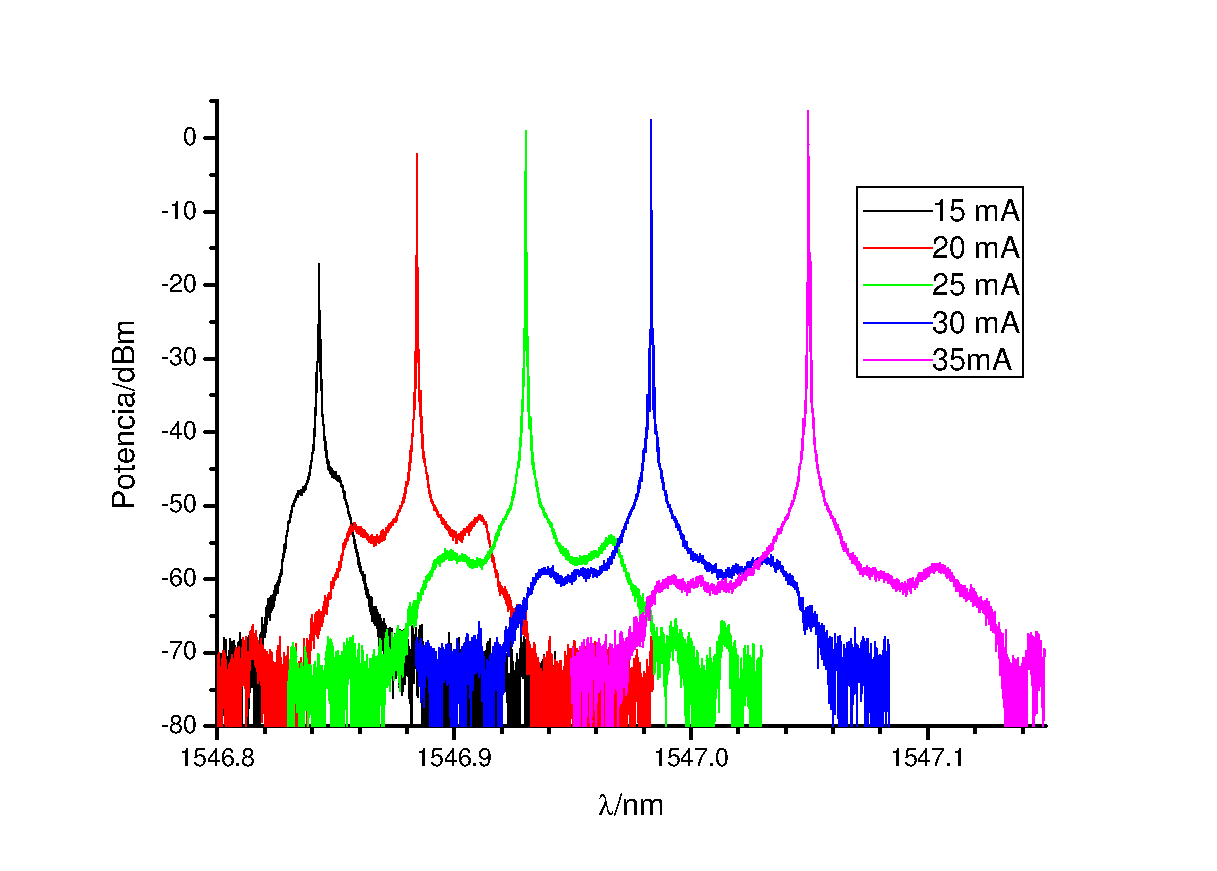
\includegraphics[width=1.0\linewidth, height=6cm]{../Chaves/OFC-GS/espectros_continua.png}
				\caption{\label{Img:spectrosCW:exp}Espectros ópticos obtenidos experimentalmente.}	
			\end{subfigure}
			\caption{\label{Img:spectrosCW}Espectros ópticos del DML para diferentes corrientes de polarización $\ibias$ obtenidos mediante simulación (izquierda \ref{Img:spectrosCW:sim}) y mediante experimento (derecha, \ref{Img:spectrosCW:exp}).}
		\end{figure}

		Comparando los espectros obtenidos mediante simulación con los obtenidos esperimentalmente se observa un gran parecido en la forma, observando una forma más puntiaguda y estrecha en los espectros con corriente $I_{bias}= 15$ mA para ambas gráficas. Además, la simulación permite observar los picos propios de las oscilaciones de relajación del láser que se observan en el experimento.

		Además, a partir de los espectros de la Figura \ref{Img:spectrosCW} se pueden obtener las longitudes de onda de los picos de emisión en función de la corriente $\ibias$. En la Tabla \ref{tab:lambdas} se muestran los valores de las longitudes de onda $lambda$ obtenidas de los espectros de la Figura \ref{Img:spectrosCW} tanto para la simulación como para el experimento.

		% tab:lambdas
		\begin{table}[H]
			\centering
			\begin{tabular}{c c c}
				\hline
				$\ibias$ & $\lambda_{sim}$ & $\lambda_{exp}$ \\\hline 
				15 & 1546.86 & 1546.84 \\
				20 & 1546.90 & 1546.88 \\
				25 & 1546.94 & 1546.93 \\
				30 & 1546.99 & 1546.98 \\
				35 & 1547.05 & 1547.05 \\\hline
			\end{tabular}
			\caption{\label{tab:lambdas}Longitud de onda de las lineas de emisión del DML en función de la $\ibias$ obtenidas de la figura \ref{Img:spectrosCW}. Se muestran los valores experimentales $\lambda_{exp}$ obtenidos de la gráfica \ref{Img:spectrosCW:exp} con un error de $\delta\lambda_{exp} = 0.02$, y los valores obtenidos de la simulación de la gráfica \ref{Img:spectrosCW:sim}.}
		\end{table}

	Los valores de las longitudes de onda que se muestran en la Tabla \ref{tab:lambdas} muestran una gran similitud entre los valores experimentales y los obtenidos mediante simulación, obteniendo una discrepancia máxima de $0.02$ nm. De esta forma, la gran concordancia entre los valores de $\lambda$ experimentales y los obtenidos a partir de la simulación, junto con la gran similitud en la forma de los espectros, muestra la capacidad de la simulación de reproducir computacionalmente los resultados obtenidos experimentalmente en el laboratorio.

	Para el estudio de la inyección de luz se trabajará con una corriente $I_{bias} = 35$ mA. Por tanto, la Tabla \ref{tab:lambdas} permite obtener su longitud de onda de emisión de $\lambda = 1547.05$ nm, siendo además la misma que la obtenida en el experimento.

\addtocontents{toc}{\vspace{0.1cm}}
\subsection{Oscilaciones de Relajación}
	\label{Sol:CW:RoF}

	Para que el láser comience a emitir se ha de cumplir que la emisión estimulada domine frente a la emisión espontánea. Esto se produce cuando la densidad de portadores de carga en la región activa supera un valor umbral, $N_{th}$, a partir del cuál el láser comienza a emitir fotones. Si la inyección de corriente que se le aplica al láser es constante (\cw), la densidad de portadores de carga tenderá a estabilizarse en $N_{th}$. De el mismo modo, la densidad de fotones y el chirp se estabilizarán para valores $S_{th}$ y $\Phi_{th}$.

	No obstante, si se parte de unas condiciones iniciales del láser con valores $N(t=0) < N_{th}$, será necesario que transcurra un cierto tiempo hasta que el láser alcance el equilibrio y se estabilice. A este tiempo se le denomina transitorio.

	Cabe destacar que, tal y como se comentó en el apartado \ref{Mdl:Code:Trans}, para la simulación se ha trabajado con un tiempo de transitorio $t_{trans} = 1.2$ ns, en el cuál se ha operado con la raiz cuadrada del módulo de $S$ en los términos de ruido para evitar resultados complejos, despeciando dicho intervalo en el estudio de los espectros. Sin embargo, en este apartado se estudiarán las ecuaciones de balance en el transitorio para corriente continua. El trabajar con una corriente continua mayor que la corriente umbral permite disminuir el intervalo de tiempo en el que se operará con $\sqrt{|S|}$ hasta los 0.2 ns, pudiendo realizar un estudio más riguroso de las ecuaciones de balance en el transitorio.

	Se considerará una intensidad de corriente $I(t)$ función escalón con $I(t>0) = \ibias$. En la ecuación \ref{eq:transient} se muestra la función escalón $I(t)$ utilizada así como las condiciones iniciales para la densidad de portadores de carga $N(0)$, la densidad de fotones $S(0)$ y de la fase óptica $\Phi(0)$.

		%eq:transient
		\begin{equation}
			\begin{matrix}
					I(t) = \left\{\begin{matrix}
									0 & t \leq 0\\ 
									\ibias = 30 \textrm{ mA} & t > 0
							\end{matrix}\right.
					& & & & & & 
					\begin{matrix}
						N(0) = N_{tr} \\ S(0) = 10^{15} \textrm{m}^{-3}\\ \Phi(0) = 0
					\end{matrix}
				\end{matrix}
			\label{eq:transient}
		\end{equation}

	En la Figura \ref{Img:transitorio} se muestra la evolución temporal de la \I\ junto con los valores obtenidos en la simulación para la \n\, la \s\ y la \fase\ para el transitorio $t_{trans} = 1.2$ ns.

		% Img:transitorio
		\begin{figure}[H]
			\centering
			\includegraphics[width=0.7\linewidth]{transitorio.png}
			\caption{\label{Img:transitorio}Evolución temporal de la \I, la \s, la \n\ y del \chirp\ durante el transitorio. Para la \I\ se ha marcado la corriente umbral del láser $I_{th} = 14.8$ mA con una línea horizontal discontinua.}	
		\end{figure}
		
		Se observan en las evoluciones temporales de \n, \s\ y \fase\ de la Figura \ref{Img:transitorio} tres regiones diferentes en función del comportamiento de las tres magnitudes: $i$) Una vez que la corriente inyectada supera la corriente umbral $I_{th}$ (en $t=0$) la \n\ comienza a aumentar. No obstante, el valor de $N(t)$ se mantiene inferior a $N_{th}$ por lo que no se produce emisión estimulada, y así, la densidad de fotones no aumenta y toma valores aleatorios, debido a la emisión espontánea, alrededor de $S(0)$. Esto también se puede observar en el comportamiento también aleatorio del \chirp. $ii$) La \n\ continua aumentando alcanzando el valor umbral $N_{th}$ en $t = 0.23$ ns. En este punto la densidad de fotones comienza a aumentar debido a la emisión estimulada producida al superar $N_{th}$. Sin embargo, al encontrarse $S(t)$ por debajo de $S_{th}$, $N(t)$ continua creciendo tomando valores por encima $N_{th}$ hasta que $S(t)$ alcanza el valor de $S_{th}$, en $t \approx 0.37$ ns. Al alcanzar $S(t)$ el valor de $S_{th}$, comienza a dominar la emisión estimulada frente a la emisión espontánea. Al alcanzar el valor $S_{th}$ la emisión estimulada domina frente a la emisión espontánea, como se puede observar el \chirp, y la densidad de portadores de carga comienza a disminuir, alcanzando la \n\ y \chirp\ un máximo. La densidad de fotones continúa aumentando y la densidad de portadores de carga disminuyendo, llegando nuevamente a tomar valores por debajo de $N_{th}$. Debido a ésto $S(t)$ alcanza un máximo cuando $N(t) = N_{th}$ y comienza a disminuir, volviendo a tomar valores inferiores a $S_{th}$ y así, volviendo a aumentar $N(t)$. Estas oscilaciones entorno a los valores umbrales continuan, disminuyendo su amplitud, realizando un comportamiento anarmónico y se las conoce como oscilaciones de relajación. En la figura \ref{Img:transitorio} se observan claramente estas oscilaciones, siendo iguales en el tiempo para \n\ y para el \chirp\ (máximos en el mismo tiempo $t$). También se observa la relación entre las oscilaciones de estas magnitudes con las de $S(t)$, obteniendo un máximo en $S(t)$ cuando $N(t) = N_{th}$ de tal forma que ambas oscilaciones tengan el mismo periodo. $ii$) Las oscilaciones de relajación van disminuyendo a medida que el tiempo avanza alcanzando el equilibrio en el que las tres magnitudes se mantienen constante.

		A partir de los datos de la figura \ref{Img:transitorio} se pueden obtener las frecuencias de las oscilaciones de relajación en el transitorio, a patir del tiempo entre los máximos. Una primera estimación permite obtener una frecuencia de oscilación de $\nu_{RoF} \approx 5.9$ GHz, que pasado a longitud de onda equivale a $\lambda = 0.05$ nm. Comparando dicho valor con los picos debidos a las oscilaciones de relajación de los espectros para $I = 30$ mA de la figura \ref{Img:spectrosCW} observamos que se encuentran en el mismo orden de magnitud, mostrando una gran concordancia entre la simulación y el experimento.


	\addtocontents{toc}{\vspace{0.1cm}}
	\section{OFC (Gain-Switching)}
		\label{Sol:OFC}

		
Para el estudio del m\'etodo de generaci\'on de OFC mediante \gs\ se ha trabajado con una corriente de inyecci\'on $I(t)$ modulada mediante una función sinusoidal superpuesta a una corriente de polarización $\ibias$ tal y como se muestra en la ecuación \ref{eq:gainSwtching}.

	\begin{equation}
		I(t) = \ibias + \frac{2\sqrt{2}V_{RF}}{Z_0+Z_l} \sin(2\pi f_R t)
		\label{eq:gainSwtching}
	\end{equation}

	Tal y como se vi\'o en el apartado \ref{Intr:OFC:GS} la calidad del \gs\ viene dada tanto por la intensidad de los picos como por la duraci\'on del pulso. De esta manera, se ha procedido a caracterizar los peines \'opticos de frecuencia en funci\'on del \gs\ aplicado modificando la frecuencia de oscilaci\'on y la amplitud de la corriente inyectada. Para el estudio del \gs\ en función de la frecuencia de oscilaci\'on se ha modificado el valor de $f_R$, estudiando primero los OFC para altas frecuencias ($f_R = 5.0$ GHz) y luego para bajas frecuencias ($f_R = 500$ MHz). Cabe destacar que al variar el valor de la frecuencia de oscilaci\'on $f_R$, la impedancia del l\'aser $Z_l$ tambi\'en cambia y as\'i también la suma $Z_0 + Z_l$.

	Para ambos valores de frecuencias $f_R$ se han estudiado los efectos producidos al variar la amplitud de la corriente de inyecci\'on, comparando tanto los espectros ópticos obtenidos como las variables dinámicas para diferentes amplitudes. Para el estudio con diferentes amplitudes ha bastado con modificar los valores de $V_{RF}$, ya que $(Z_0 + Z_l)$ solo varia para la frecuencia.

	\addtocontents{toc}{\vspace{0.1cm}}
	\subsection{Efecto de la amplitud de modulación a altas frecuencias}
		\label{Sol:OFC:HgFreq}

		Para el estudio del efecto de la amplitud de modulación a altas frecuencias se ha trabajado con una corriente de polarización $\ibias = 30$ mA y una frecuencia $f_R = 5.0$ GHz. Tal y como se vi\'o en el apartado \ref{Sol:CW:RoF}, la frecuencia de oscilaciones de relajación del l\'aser para $\ibias = 30$ mA es de $\nu_{RoF} \approx 5.9$ GHz, del orden de $f_R$. Se han resulto las ecuaciones de balance, obteniendo los OFC para tres amplitudes diferentes con $V_{RF}$: $0.05$ V, $1.00$ V y $1.50$ V. 

		En la Figura \ref{Img:rateEquations} se muestra la evolución temporal de la \I, la \s, la \n\ y de \chirp\ para varios valores de $V_{RF}$ pasada la zona del transitorio.

			% Img:rateEquations
			\begin{figure}[H]
				\centering
				\includegraphics[width=1.0\linewidth]{rateEquations.png}
				\caption{\label{Img:rateEquations}Evolución temporal de la \I ((a)-(c)), la \s ((d)-(f)), la \n\ ((g)-(i)) y del \chirp\ ((j)-(l)) en funci\'on de $V_{RF}$ pasada la zona del transitorio. Para la \I\ se ha marcado la corriente umbral del l\'aser $I_{th} = 14.8$ mA con una l\'inea horizontal discontinua. En la primera columna se muestran las evoluciones temporales para una amplitud de la corriente equivalente a $V_{RF} = 0.05$ V (verde), en la segunda columna para $V_{RF} = 1.00$ V (azul) y en la tercera columna de $V_{RF} = 1.50$ V(naraja).}	
			\end{figure}

		Mientras que para el caso del l\'aser en corriente continua ($I(t) = \ibias$) estudiado en la secci\'on anterior (secci\'on \ref{Sol:CW}), $S(t)$, $N(t)$ y el \chirp\ alcanzaban un valor constante pasado el transitorio, ahora la modulación en la corriente produce oscilaciones de igual periodo en $S(t)$, $N(t)$ y el \chirp. Se observa un aumento de la amplitud en $S(t)$, $N(t)$ y el \chirp\ al aumentar la amplitud de la corriente. Adem\'as, se observa como las oscilaciones en $N(t)$ y el \chirp\ van en fase (m\'aximos en el mismo tiempo $t$), mientras que los m\'aximos de $S(t)$ se obtienen cuando $N(t)$ decae a $N_{th}$.
			
		Para el caso de $V_{RF} = 0.05$ V, con una menor amplitud, se observa que las oscilaciones en la corriente (Figura \ref{Img:rateEquations} (a)) son pequeñas. Al igual que la corriente; la \s, la \n\ y el \chirp\ tambi\'en presentan oscilaciones de amplitud pequeña.% Cabe destacar que para este caso de amplitud pequeña, la \s\ (Figura \ref{Img:rateEquations} (d)) toma valores cercanos a cero, al no producirse ning\'un pico de intensidad. Esto produce que la emisi\'on estimulada no tome valores suficientemente altos como para que la emisi\'on espont\'anea sea despreciable y as\'i, se puede observar en el \chirp\ (Figura \ref{Img:rateEquations} (g)) el ruido debido a la emisión espont\'anea.

		Al aumentar la amplitud de la corriente a $V_{RF} = 1$ V (Figura \ref{Img:rateEquations} (b)) se observa como los aumentos de la corriente durante la oscilaci\'on coinciden con el crecimiento de \n\ (Figura \ref{Img:rateEquations} (k)), haciendo que tome valores muy superiores a $N_{th}$. A su vez, esto produce que, al superar $N(t)$ el valor del umbral $N_{th}$, la \s\ (Figura \ref{Img:rateEquations} (e)) tambi\'en tenga un pico superior al valor del l\'aser en corriente continua. De igual forma que ocurria en el transitorio, al aumentar $S(t)$ y dominar la emisi\'on estimulada, $N(t)$ comienza a disminuir, alcanzando un m\'aximo. Sin embargo, en el momento en el que $N(t)$ alcanza el m\'inimo, la corriente se encuentra por debajo de la corriente umbral $I_{th}$, y $N(t)$ no puede aumentar hasta que $I(t)$ toma nuevamente valores mayores de $I_{th}$. Debido a este tiempo $t$ en el que $N(t)$ no es capaz de volver a aumentar, compensando la disminuci\'on de \s, hay un mayor tiempo $t$ en el que $S(t)$ es cero, y as\'i no hay emisi\'on estimulada. Esta alternancia entre el dominio de la emisi\'on estimulada y la emisi\'on espont\'anea se puede pareciar en el \chirp\ (Figura \ref{Img:rateEquations} (h)), en la que se aprecia el ruido debido a la emisión espont\'anea cuando la densidad de fotones es cero, mienstras que durante los picos de $S(t)$ el ruido es despreciable y no se observa.
			
		Para la amplitud de $V_{RF} = 1.5$ V se observa la misma tendencia que para $V_{RF} = 1$ V, a excepci\'on de que en este caso, al aumentar la amplitud aumenta el tiempo en el que la corriente es menor que $I_{th}$ y as\'i el tiempo en el que $S(t)$ es cero y domina la emisi\'on espontánea.


		En la Figura \ref{Img:PSD} se muestran los espectros de los OFC obtenidos mediante \gs\ para las tres amplitudes de la Figura \ref{Img:rateEquations}.

			% Img:PSD
			\begin{figure}[H]
				\centering
				\includegraphics[width=1.0\linewidth]{PSD.png}
				\caption{\label{Img:PSD}Espectros de los OFC obtenidos mediante \gs\ para $\ibias = 30$ mA, $f_R = 5$ GHz y amplitud de modulaci\'on $V_{RF} = 0.05$ V (verde), $1.00$ V (azul) y $1.50$ V (naranja).}
			\end{figure}
			
		Al igual que se obtuvo en la Figura \ref{Img:rateEquations}, se puede observar como el caso de la amplitud de modulaci\'on $V_{RF} = 0.05$ V se asemeja al del l\'aser en corriente cont\'inua, obteniendo un espectro (Figura \ref{Img:PSD} (verde)) con la frecuencia de emisi\'on dominante de la Figura \ref{Img:spectrosCW}. Como consecuencia del \gs\ realizado se observan excitadas las frecuencias de emisi\'on, apareciendo nuebas l\'ineas de emisi\'on a los lados de la emisi\'on principal.

		Para el caso de $V_{RF} = 1$ V se observa un OFC (Figura \ref{Img:PSD} (azul)) de gran calidad formado por numerosas l\'ineas de emisión equiespaciadas y bien definidas. Se ha obtenido una regi\'on de longitudes de onda con l\'ineas de emisión de la misma densidad espectral de potencia lo cuál resulta enuna gran calidad del OFC.

		Por otro lado, se observa que para el caso de $V_{RF} = 1.5$ V (Figura \ref{Img:PSD} (naranja)) el OFC se detruye debido al ruido de la emisión espont\'anea, obteniendo l\'ineas de emisión poco definidas, con un espaciado variado y mucho ruido.

		De esta forma, se ha podido caracterizar la calidad de los OFC, y del \gs, para altas frecuencias en función de la amplitud de modulaci\'on. Se ha podido observar la creaci\'on del OFC para $V_{RF} = 1$ V, as\'i como la destrucci\'on de este para altas amplitudes, con $V_{RF} = 1.5$ V.

		Tal y como se ha comentado a partir de los resultados de la Figura \ref{Img:rateEquations}, uno de los efectos de aumentar la amplitud de modulaci\'on es la disminuci\'on de la corriente por debajo de $I_{th}$ por un tiempo $t$, que aumenta con la amplitud. Sin embargo, \'esto también se puede controlar para una amplitud fija, variando la corriente de polarizaci\'on $\ibias$.

		En la Figura \ref{Img:current} se muestran la potencia $P(t)$, obtenida a partir de la \s\ \ref{eq:Power}, y los espectros de los OFC con $f_R = 5$ GHz, $V_{RF} = 1$ V e $\ibias = 30$ mA y $50$ mA.

			% Img:current
			\begin{figure}[H]
				\centering
				\includegraphics[width=1.0\linewidth]{current.png}
				\caption{\label{Img:current}Perfil temporal de las potencias $P(t)$ (izquierda) y espectros (derecha) de OFC con $f_R = 5$ GHz, $V_{RF} = 1$ V e $\ibias = 30$ mA (azul) y $50$ mA (naranja).}	
			\end{figure}

		En el perfil temporal de la potencia $P(t)$ de $\ibias = 30$ mA (Figura \ref{Img:current} (izquierda, azul)) se observan las zonas de tiempo con $P(t) \propto S(t) = 0$ vistas en la Figura \ref{Img:rateEquations}, debidas a que la corriente toma valores por debajo de $I_{th}$ y as\'i \n\ no puede aumentar. De igual manera se ha obtenido un OFC de gran calidad (Figura \ref{Img:current} (derecha, azul)) como el obtenido en la Figura \ref{Img:PSD}.

		Sin embargo, en el caso de $\ibias = 50$ mA, al aumentar la corriente de polarizaci\'on, \'esta desplaza la función sinusoidal de la intensidad alejandola de $I_{th}$ y as\'i la amplitud de modulaci\'on no es suficiente para llegar a cruzar $I_{th}$. Esto se puede observar en que el perfil temporal de $P(t)$ (Figura \ref{Img:current} (izquierda, naranja)) no toma nunca el valor cero y as\'i realiza oscilaciones completas. Puesto que la frecuencia $f_R$ y la amplitud $V_{RF}$ de modulación s\'i son suficientes com para que se d\'e \gs, se observa un espectro (Figura \ref{Img:current} (derecha, naranja)) con un OFC formado por l\'ineas bien definidas e igualmente espaciadas. No obstante, el OFC obtenido para $\ibias = 50$ mA es m\'as estrecho que el obtenido para $\ibias = 30$ mA, careciendo de una meseta bien definida con l\'ineas de emisi\'on con densidad espectral de potencia similar. Debido a esto, el OFC obtenido para $\ibias = 30$ mA es de mayor calidad que el obtenido para $\ibias = 50$ mA.

		Otro de los efectos de aumentar la $\ibias$ de tal manera que no cruce la $I_{th}$ es la falta de una regi\'on donde domine la emisi\'on espont\'anea, como ocurria en la Figura \ref{Img:rateEquations}. Esto se puede observar en el menor ruido obtenido en el espectro para $\ibias = 50$ mA (Figura \ref{Img:current} (derecha, naranja)) frente al obtenido en el espectro de $\ibias = 30$ mA (Figura \ref{Img:current} (derecha, azul)).

	\addtocontents{toc}{\vspace{0.1cm}}
	\subsection{Efecto de la amplitud de modulación a bajas frecuencias}
		\label{Sol:OFC:LwFreq}

		Para el estudio del efecto de la amplitud de modulación a bajas frecuencias se ha trabajado con una corriente de polarización $\ibias = 50$ mA y una frecuencia $f_R = 500$ MHz. Se han obtenido la potencia $P(t)$ y los OFC para cuatro amplitudes diferentes, tomando cuatro valores distintos para $V_{RF}$: $0.05$ V, $0.4$ V, $1.0$ V y $1.2$ V.

		En la Figura \ref{Img:500} se muestran los perfiles temporales de la potencia $P(t)$ y los espectros de los OFC para $\ibias = 50$ mA, $f_R = 500$ MHz y $V_{RF} = 0.05$ V, $0.4$ V, $1.0$ V y $1.2$ V.
			% Img:500
			\begin{figure}[H]
				\centering
				\includegraphics[width=1.0\linewidth]{500.png}
				\caption{\label{Img:500}Perfiles temporales de la potencia $P(t)$ (fila superior) y espectros (fila inferior) de los OFC para $\ibias = 50$ mA, $f_R = 500$ MHz y $V_{RF} = 0.05$ V (primera columna), $0.4$ V (segunda columna), $1.0$ V (tercera columna) y $1.2$ V (cuarta columna).}	
			\end{figure}

		Al igual que se obtuvo en el apartado anterior para el caso de altas frecuencias con $\ibias = 50$ mA (Figura \ref{Img:current}), se observan en la Figura \ref{Img:500} perfiles temporales de la potencia oscilantes entorno al valor de la potencia en corriente continua ($P_{CW} \approx 4.7$ mW), variando su amplitud en funci\'on de la amplitud de modulación. Al tener una $\ibias$ muy superior a $I_{th}$ y una frecuencia baja, la amplitud de modulaci\'on no permite mantener la corriente de inyecci\'on por debajo de la corriente umbral un tiempo suficiente como para que $P(t) \propto S(t) = 0$, tal y como se observa en las Figuras \ref{Img:500} (fila superior).

		Para el caso de la amplitud de modulaci\'on pequeña con $V_{RF} = 0.05$ V, se ha obtenido un comportamiento muy similar a la corriente continua, al igual que para altas frecuencias. El espectro obtenido para esta amplitud de modulaci\'on es similar al de la Figura \ref{Img:PSD} (verde) del apartado anterior, obteniendo un pico de emisi\'on dominante correpondiente a la emisi\'on en continua y dos picos a cada lado debidos a la excitaci\'on de la frecuencia de oscilación.

		Se observa como, al igual que ocurria en a altas frecuencias, a medida que aumenta la amplitud de modulación aumenta el n\'umero de l\'ineas de emisión de espectro, llegando a destruirse para altas amplitudes de modulación. Sin embargo, al trabajar a bajar frecuencias se observa una clara irregularidad en el perfil del OFC, tomando los picos valores muy diversos de la densidad espectral de potencia. Esto implica una perdida de la calidad de los OFC a bajas frecuencias con respecto a altas frecuencias. 

		DEBERIA HABLAR SOBRE LOS PICOS QUE SE OBSERVAN EN LA POTENCIA PARA V = 1.2

		En la Figura \ref{Img:500mhz} se muestran los perfiles temporales de la potencia $P(t)$ y los espectros de los OFC para $\ibias = 50$ mA, $f_R = 500$ MHz y $V_{RF} = 0.1$ V, $0.4$ V, $1.2$ V y $1.6$ V obtenidos experimentalmente \cite{Chaves19}.

			% Img:500mhz
			\begin{figure}[H]
				\centering
				\includegraphics[width=1.0\linewidth]{../Chaves/OFC-GS/500mhz.png}
				\caption{\label{Img:500mhz}Perfiles temporales de la potencia $P(t)$ (fila superior) y espectros (fila inferior) de los OFC para $\ibias = 50$ mA, $f_R = 500$ MHz y $V_{RF} = 0.1$ V (primera columna), $0.4$ V (segunda columna), $1.2$ V (tercera columna) y $1.6$ V (cuarta columna) obtenidos experimentalmente \cite{Chaves19}.}	
			\end{figure}

		En la Figura \ref{Img:500mhz} se muestran la potencia $P(t)$ y los espectros experimentales para diferentes amplitudes de modulación, permitiendo comparar los resultados obtenidos mediante simulación con los obtenidos en el laboratorio.

		En la cuarta columna de la Figura \ref{Img:500mhz} se muestran los resultados obtenidos para una amplitud de $V_{RF} = 1.6$ V, observando como el espectro de frecuencia se encuentra completamente destruido. Dichos resultados no pudieron ser obtenidos mediante la simulación debido al problema en el transitorio con $\sqrt{S(t)}$. En la primera columna de la Figura \ref{Img:500mhz} se muestran los resultados para una amplitud de modulación pequeña de $V_{RF} = 0.1$ V. Al igual que en los resultados de la simulación, se obtiene un comportamiento similar al de la corriente continua con un pico de emisi\'on dominante. No obstante, al tratarse de el doble de la amplitud utilizada en la simulaci\'on de la Figura \ref{Img:500} se obtienen un mayor n\'umero de picos de emisión estimulados. Los resultados que se muestran en la segunda columna de la Figura \ref{Img:500mhz}  para $V_{RF} = 0.4$ V equivalen a los resultados de la simulación de la segunda columna de la Figura \ref{Img:500}. En ambas figuras se pueden observar un OFC con un perfil aproximandamente sim\'etico con un pico de menor intensidad en el centro. Por \'ultimo, la tercera columna de la Figura \ref{Img:500mhz} equivale a la cuarta columna de la Figura \ref{Img:500}. Ambos espectros presentan un perfil similar con un aumento brusco de la densidad espectral de potencia de los picos para bajas longitudes de onda, seguido de una disminuci\'on m\'as tenue para lontitudes de onda mayores. Ambos perfiles temporales de potencia presentan LOS PICOS DE LOS QUE HE DE HABLAR.

	El excelente acuerdo entre los resultados de la simulaci\'on de la Figura \ref{Img:500} y los resultados experimentales de la Figura \ref{Img:500mhz} indican la capacidad de la simulaci\'on de explicar los procesos que involucra el \gs\ en la generaci\'on de OFC, pudiendo servir para la caracterizaci\'on de la calidad de los OFC.




			\addtocontents{toc}{\vspace{0.01cm}}
			\chapter{Láser en solitario}
				\label{Sol}

				\graphicspath{{../Graphics/Cpt1-Charactz/}}

\newcommand{\cw}{corriente continua}

Antes de abordar el estudio de la dinámica no lineal del láser de semiconductor de modo discreto se ha realizado la simulación del láser en solitario, sin inyección de luz del láser esclavo ($P_{Iny} = 0$). Se han realizado simulaciones para el láser tanto en \cw\ (CW de sus siglas en inglés), como en Gain-Switching, comparando los resultados con los obtenidos experimentalmente en condiciones similares \cite{Chaves19}.

	\addtocontents{toc}{\vspace{0.1cm}}
	\section{Láser en \cw}
		\label{Sol:CW}
		
		
Para poder realizar las simulaciones en \cw\ se ha trabajado con una corriente de inyección constante e igual a la corriente de polarización ($I(t) = I_{bias}$), tomando $V_{RF} = 0$.

HABLAR DE QUE EN CONTINUA SE TIENE QUE $\frac{\mathrm{d} N}{\mathrm{d} t} = \frac{\mathrm{d} S}{\mathrm{d} t} = \frac{\mathrm{d} \Phi}{\mathrm{d} t} = 0$

\addtocontents{toc}{\vspace{0.1cm}}
\subsection{Espectros de emisión}
	\label{Sol:CW:Spectr}

	Tal y como se vio en la sección \ref{Intr:LsrSmcdtr}, pequeñas variaciones en la corriente de inyección del láser producen desplazamientos de la línea de emisión del láser en el espectro de frecuencias. Por ello es importante conocer el valor de la longitud de onda del pico de emisión del láser en solitario en función de la corriente de polarización $\ibias$, de cara a realizar el estudio de la inyección de luz.

	En la Figura \ref{Img:spectrosCW} se muestran las densidades espectrales de potencia del láser a diferentes corrientes de polarización, comparando los datos obtenidos mediante la simulación del láser(Figura \ref{Img:spectrosCW:sim}), con los obtenidos experimentalmente(Figura \ref{Img:spectrosCW:exp}).

		% Img:spectrosCW {Img:spectrosCW:sim, Img:spectrosCW:exp}
		\begin{figure}[H]
			\centering
			\begin{subfigure}{0.45\textwidth}
				\centering
				\includegraphics[width=1.0\linewidth, height=6cm]{Espectros.png}
				\caption{\label{Img:spectrosCW:sim}Espectros ópticos obtenidos mediante simulación.}
			\end{subfigure}
			\begin{subfigure}{0.45\textwidth}
				\centering
				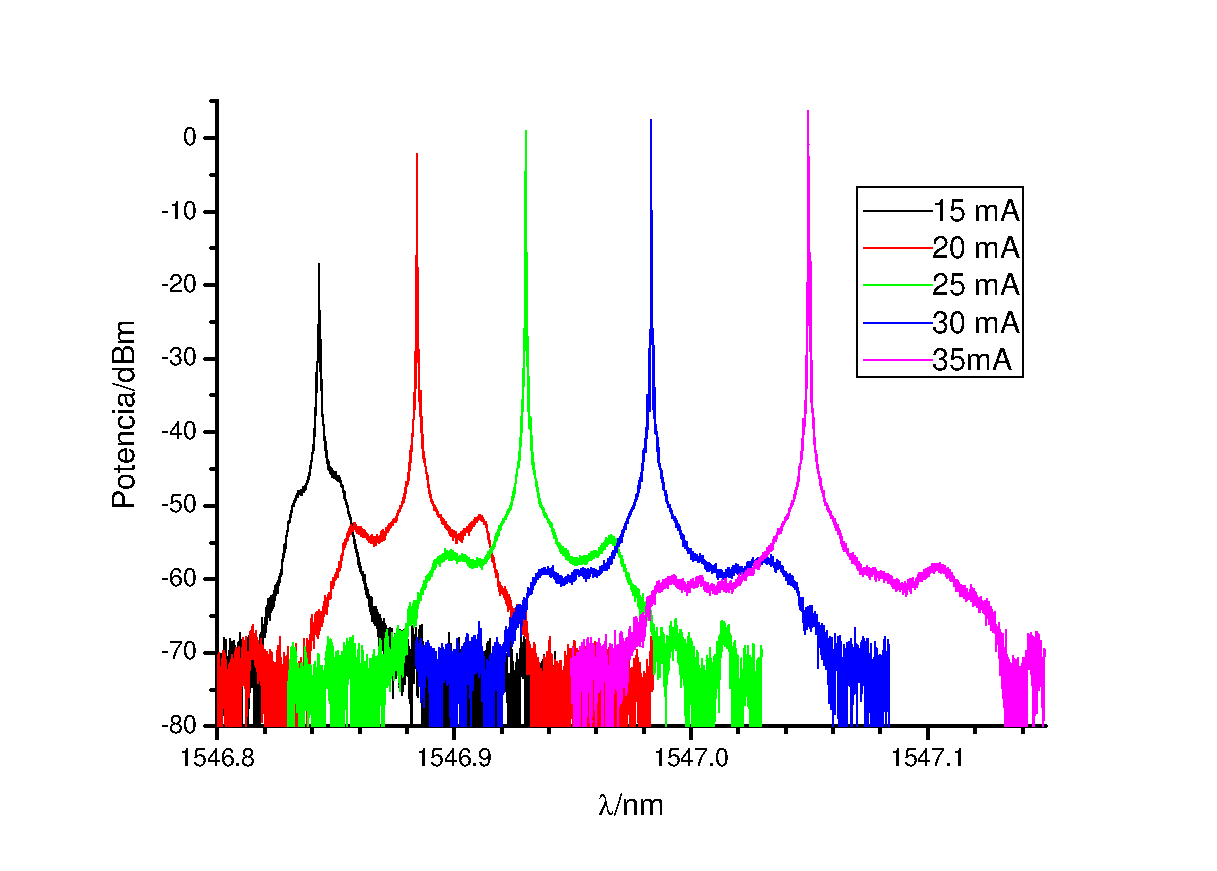
\includegraphics[width=1.0\linewidth, height=6cm]{../Chaves/OFC-GS/espectros_continua.png}
				\caption{\label{Img:spectrosCW:exp}Espectros ópticos obtenidos experimentalmente.}	
			\end{subfigure}
			\caption{\label{Img:spectrosCW}Espectros ópticos del DML para diferentes corrientes de polarización $\ibias$ obtenidos mediante simulación (izquierda \ref{Img:spectrosCW:sim}) y mediante experimento (derecha, \ref{Img:spectrosCW:exp}).}
		\end{figure}

		Comparando los espectros obtenidos mediante simulación con los obtenidos esperimentalmente se observa un gran parecido en la forma, observando una forma más puntiaguda y estrecha en los espectros con corriente $I_{bias}= 15$ mA para ambas gráficas. Además, la simulación permite observar los picos propios de las oscilaciones de relajación del láser que se observan en el experimento.

		Además, a partir de los espectros de la Figura \ref{Img:spectrosCW} se pueden obtener las longitudes de onda de los picos de emisión en función de la corriente $\ibias$. En la Tabla \ref{tab:lambdas} se muestran los valores de las longitudes de onda $lambda$ obtenidas de los espectros de la Figura \ref{Img:spectrosCW} tanto para la simulación como para el experimento.

		% tab:lambdas
		\begin{table}[H]
			\centering
			\begin{tabular}{c c c}
				\hline
				$\ibias$ & $\lambda_{sim}$ & $\lambda_{exp}$ \\\hline 
				15 & 1546.86 & 1546.84 \\
				20 & 1546.90 & 1546.88 \\
				25 & 1546.94 & 1546.93 \\
				30 & 1546.99 & 1546.98 \\
				35 & 1547.05 & 1547.05 \\\hline
			\end{tabular}
			\caption{\label{tab:lambdas}Longitud de onda de las lineas de emisión del DML en función de la $\ibias$ obtenidas de la figura \ref{Img:spectrosCW}. Se muestran los valores experimentales $\lambda_{exp}$ obtenidos de la gráfica \ref{Img:spectrosCW:exp} con un error de $\delta\lambda_{exp} = 0.02$, y los valores obtenidos de la simulación de la gráfica \ref{Img:spectrosCW:sim}.}
		\end{table}

	Los valores de las longitudes de onda que se muestran en la Tabla \ref{tab:lambdas} muestran una gran similitud entre los valores experimentales y los obtenidos mediante simulación, obteniendo una discrepancia máxima de $0.02$ nm. De esta forma, la gran concordancia entre los valores de $\lambda$ experimentales y los obtenidos a partir de la simulación, junto con la gran similitud en la forma de los espectros, muestra la capacidad de la simulación de reproducir computacionalmente los resultados obtenidos experimentalmente en el laboratorio.

	Para el estudio de la inyección de luz se trabajará con una corriente $I_{bias} = 35$ mA. Por tanto, la Tabla \ref{tab:lambdas} permite obtener su longitud de onda de emisión de $\lambda = 1547.05$ nm, siendo además la misma que la obtenida en el experimento.

\addtocontents{toc}{\vspace{0.1cm}}
\subsection{Oscilaciones de Relajación}
	\label{Sol:CW:RoF}

	Para que el láser comience a emitir se ha de cumplir que la emisión estimulada domine frente a la emisión espontánea. Esto se produce cuando la densidad de portadores de carga en la región activa supera un valor umbral, $N_{th}$, a partir del cuál el láser comienza a emitir fotones. Si la inyección de corriente que se le aplica al láser es constante (\cw), la densidad de portadores de carga tenderá a estabilizarse en $N_{th}$. De el mismo modo, la densidad de fotones y el chirp se estabilizarán para valores $S_{th}$ y $\Phi_{th}$.

	No obstante, si se parte de unas condiciones iniciales del láser con valores $N(t=0) < N_{th}$, será necesario que transcurra un cierto tiempo hasta que el láser alcance el equilibrio y se estabilice. A este tiempo se le denomina transitorio.

	Cabe destacar que, tal y como se comentó en el apartado \ref{Mdl:Code:Trans}, para la simulación se ha trabajado con un tiempo de transitorio $t_{trans} = 1.2$ ns, en el cuál se ha operado con la raiz cuadrada del módulo de $S$ en los términos de ruido para evitar resultados complejos, despeciando dicho intervalo en el estudio de los espectros. Sin embargo, en este apartado se estudiarán las ecuaciones de balance en el transitorio para corriente continua. El trabajar con una corriente continua mayor que la corriente umbral permite disminuir el intervalo de tiempo en el que se operará con $\sqrt{|S|}$ hasta los 0.2 ns, pudiendo realizar un estudio más riguroso de las ecuaciones de balance en el transitorio.

	Se considerará una intensidad de corriente $I(t)$ función escalón con $I(t>0) = \ibias$. En la ecuación \ref{eq:transient} se muestra la función escalón $I(t)$ utilizada así como las condiciones iniciales para la densidad de portadores de carga $N(0)$, la densidad de fotones $S(0)$ y de la fase óptica $\Phi(0)$.

		%eq:transient
		\begin{equation}
			\begin{matrix}
					I(t) = \left\{\begin{matrix}
									0 & t \leq 0\\ 
									\ibias = 30 \textrm{ mA} & t > 0
							\end{matrix}\right.
					& & & & & & 
					\begin{matrix}
						N(0) = N_{tr} \\ S(0) = 10^{15} \textrm{m}^{-3}\\ \Phi(0) = 0
					\end{matrix}
				\end{matrix}
			\label{eq:transient}
		\end{equation}

	En la Figura \ref{Img:transitorio} se muestra la evolución temporal de la \I\ junto con los valores obtenidos en la simulación para la \n\, la \s\ y la \fase\ para el transitorio $t_{trans} = 1.2$ ns.

		% Img:transitorio
		\begin{figure}[H]
			\centering
			\includegraphics[width=0.7\linewidth]{transitorio.png}
			\caption{\label{Img:transitorio}Evolución temporal de la \I, la \s, la \n\ y del \chirp\ durante el transitorio. Para la \I\ se ha marcado la corriente umbral del láser $I_{th} = 14.8$ mA con una línea horizontal discontinua.}	
		\end{figure}
		
		Se observan en las evoluciones temporales de \n, \s\ y \fase\ de la Figura \ref{Img:transitorio} tres regiones diferentes en función del comportamiento de las tres magnitudes: $i$) Una vez que la corriente inyectada supera la corriente umbral $I_{th}$ (en $t=0$) la \n\ comienza a aumentar. No obstante, el valor de $N(t)$ se mantiene inferior a $N_{th}$ por lo que no se produce emisión estimulada, y así, la densidad de fotones no aumenta y toma valores aleatorios, debido a la emisión espontánea, alrededor de $S(0)$. Esto también se puede observar en el comportamiento también aleatorio del \chirp. $ii$) La \n\ continua aumentando alcanzando el valor umbral $N_{th}$ en $t = 0.23$ ns. En este punto la densidad de fotones comienza a aumentar debido a la emisión estimulada producida al superar $N_{th}$. Sin embargo, al encontrarse $S(t)$ por debajo de $S_{th}$, $N(t)$ continua creciendo tomando valores por encima $N_{th}$ hasta que $S(t)$ alcanza el valor de $S_{th}$, en $t \approx 0.37$ ns. Al alcanzar $S(t)$ el valor de $S_{th}$, comienza a dominar la emisión estimulada frente a la emisión espontánea. Al alcanzar el valor $S_{th}$ la emisión estimulada domina frente a la emisión espontánea, como se puede observar el \chirp, y la densidad de portadores de carga comienza a disminuir, alcanzando la \n\ y \chirp\ un máximo. La densidad de fotones continúa aumentando y la densidad de portadores de carga disminuyendo, llegando nuevamente a tomar valores por debajo de $N_{th}$. Debido a ésto $S(t)$ alcanza un máximo cuando $N(t) = N_{th}$ y comienza a disminuir, volviendo a tomar valores inferiores a $S_{th}$ y así, volviendo a aumentar $N(t)$. Estas oscilaciones entorno a los valores umbrales continuan, disminuyendo su amplitud, realizando un comportamiento anarmónico y se las conoce como oscilaciones de relajación. En la figura \ref{Img:transitorio} se observan claramente estas oscilaciones, siendo iguales en el tiempo para \n\ y para el \chirp\ (máximos en el mismo tiempo $t$). También se observa la relación entre las oscilaciones de estas magnitudes con las de $S(t)$, obteniendo un máximo en $S(t)$ cuando $N(t) = N_{th}$ de tal forma que ambas oscilaciones tengan el mismo periodo. $ii$) Las oscilaciones de relajación van disminuyendo a medida que el tiempo avanza alcanzando el equilibrio en el que las tres magnitudes se mantienen constante.

		A partir de los datos de la figura \ref{Img:transitorio} se pueden obtener las frecuencias de las oscilaciones de relajación en el transitorio, a patir del tiempo entre los máximos. Una primera estimación permite obtener una frecuencia de oscilación de $\nu_{RoF} \approx 5.9$ GHz, que pasado a longitud de onda equivale a $\lambda = 0.05$ nm. Comparando dicho valor con los picos debidos a las oscilaciones de relajación de los espectros para $I = 30$ mA de la figura \ref{Img:spectrosCW} observamos que se encuentran en el mismo orden de magnitud, mostrando una gran concordancia entre la simulación y el experimento.


	\addtocontents{toc}{\vspace{0.1cm}}
	\section{OFC (Gain-Switching)}
		\label{Sol:OFC}

		
Para el estudio del m\'etodo de generaci\'on de OFC mediante \gs\ se ha trabajado con una corriente de inyecci\'on $I(t)$ modulada mediante una función sinusoidal superpuesta a una corriente de polarización $\ibias$ tal y como se muestra en la ecuación \ref{eq:gainSwtching}.

	\begin{equation}
		I(t) = \ibias + \frac{2\sqrt{2}V_{RF}}{Z_0+Z_l} \sin(2\pi f_R t)
		\label{eq:gainSwtching}
	\end{equation}

	Tal y como se vi\'o en el apartado \ref{Intr:OFC:GS} la calidad del \gs\ viene dada tanto por la intensidad de los picos como por la duraci\'on del pulso. De esta manera, se ha procedido a caracterizar los peines \'opticos de frecuencia en funci\'on del \gs\ aplicado modificando la frecuencia de oscilaci\'on y la amplitud de la corriente inyectada. Para el estudio del \gs\ en función de la frecuencia de oscilaci\'on se ha modificado el valor de $f_R$, estudiando primero los OFC para altas frecuencias ($f_R = 5.0$ GHz) y luego para bajas frecuencias ($f_R = 500$ MHz). Cabe destacar que al variar el valor de la frecuencia de oscilaci\'on $f_R$, la impedancia del l\'aser $Z_l$ tambi\'en cambia y as\'i también la suma $Z_0 + Z_l$.

	Para ambos valores de frecuencias $f_R$ se han estudiado los efectos producidos al variar la amplitud de la corriente de inyecci\'on, comparando tanto los espectros ópticos obtenidos como las variables dinámicas para diferentes amplitudes. Para el estudio con diferentes amplitudes ha bastado con modificar los valores de $V_{RF}$, ya que $(Z_0 + Z_l)$ solo varia para la frecuencia.

	\addtocontents{toc}{\vspace{0.1cm}}
	\subsection{Efecto de la amplitud de modulación a altas frecuencias}
		\label{Sol:OFC:HgFreq}

		Para el estudio del efecto de la amplitud de modulación a altas frecuencias se ha trabajado con una corriente de polarización $\ibias = 30$ mA y una frecuencia $f_R = 5.0$ GHz. Tal y como se vi\'o en el apartado \ref{Sol:CW:RoF}, la frecuencia de oscilaciones de relajación del l\'aser para $\ibias = 30$ mA es de $\nu_{RoF} \approx 5.9$ GHz, del orden de $f_R$. Se han resulto las ecuaciones de balance, obteniendo los OFC para tres amplitudes diferentes con $V_{RF}$: $0.05$ V, $1.00$ V y $1.50$ V. 

		En la Figura \ref{Img:rateEquations} se muestra la evolución temporal de la \I, la \s, la \n\ y de \chirp\ para varios valores de $V_{RF}$ pasada la zona del transitorio.

			% Img:rateEquations
			\begin{figure}[H]
				\centering
				\includegraphics[width=1.0\linewidth]{rateEquations.png}
				\caption{\label{Img:rateEquations}Evolución temporal de la \I ((a)-(c)), la \s ((d)-(f)), la \n\ ((g)-(i)) y del \chirp\ ((j)-(l)) en funci\'on de $V_{RF}$ pasada la zona del transitorio. Para la \I\ se ha marcado la corriente umbral del l\'aser $I_{th} = 14.8$ mA con una l\'inea horizontal discontinua. En la primera columna se muestran las evoluciones temporales para una amplitud de la corriente equivalente a $V_{RF} = 0.05$ V (verde), en la segunda columna para $V_{RF} = 1.00$ V (azul) y en la tercera columna de $V_{RF} = 1.50$ V(naraja).}	
			\end{figure}

		Mientras que para el caso del l\'aser en corriente continua ($I(t) = \ibias$) estudiado en la secci\'on anterior (secci\'on \ref{Sol:CW}), $S(t)$, $N(t)$ y el \chirp\ alcanzaban un valor constante pasado el transitorio, ahora la modulación en la corriente produce oscilaciones de igual periodo en $S(t)$, $N(t)$ y el \chirp. Se observa un aumento de la amplitud en $S(t)$, $N(t)$ y el \chirp\ al aumentar la amplitud de la corriente. Adem\'as, se observa como las oscilaciones en $N(t)$ y el \chirp\ van en fase (m\'aximos en el mismo tiempo $t$), mientras que los m\'aximos de $S(t)$ se obtienen cuando $N(t)$ decae a $N_{th}$.
			
		Para el caso de $V_{RF} = 0.05$ V, con una menor amplitud, se observa que las oscilaciones en la corriente (Figura \ref{Img:rateEquations} (a)) son pequeñas. Al igual que la corriente; la \s, la \n\ y el \chirp\ tambi\'en presentan oscilaciones de amplitud pequeña.% Cabe destacar que para este caso de amplitud pequeña, la \s\ (Figura \ref{Img:rateEquations} (d)) toma valores cercanos a cero, al no producirse ning\'un pico de intensidad. Esto produce que la emisi\'on estimulada no tome valores suficientemente altos como para que la emisi\'on espont\'anea sea despreciable y as\'i, se puede observar en el \chirp\ (Figura \ref{Img:rateEquations} (g)) el ruido debido a la emisión espont\'anea.

		Al aumentar la amplitud de la corriente a $V_{RF} = 1$ V (Figura \ref{Img:rateEquations} (b)) se observa como los aumentos de la corriente durante la oscilaci\'on coinciden con el crecimiento de \n\ (Figura \ref{Img:rateEquations} (k)), haciendo que tome valores muy superiores a $N_{th}$. A su vez, esto produce que, al superar $N(t)$ el valor del umbral $N_{th}$, la \s\ (Figura \ref{Img:rateEquations} (e)) tambi\'en tenga un pico superior al valor del l\'aser en corriente continua. De igual forma que ocurria en el transitorio, al aumentar $S(t)$ y dominar la emisi\'on estimulada, $N(t)$ comienza a disminuir, alcanzando un m\'aximo. Sin embargo, en el momento en el que $N(t)$ alcanza el m\'inimo, la corriente se encuentra por debajo de la corriente umbral $I_{th}$, y $N(t)$ no puede aumentar hasta que $I(t)$ toma nuevamente valores mayores de $I_{th}$. Debido a este tiempo $t$ en el que $N(t)$ no es capaz de volver a aumentar, compensando la disminuci\'on de \s, hay un mayor tiempo $t$ en el que $S(t)$ es cero, y as\'i no hay emisi\'on estimulada. Esta alternancia entre el dominio de la emisi\'on estimulada y la emisi\'on espont\'anea se puede pareciar en el \chirp\ (Figura \ref{Img:rateEquations} (h)), en la que se aprecia el ruido debido a la emisión espont\'anea cuando la densidad de fotones es cero, mienstras que durante los picos de $S(t)$ el ruido es despreciable y no se observa.
			
		Para la amplitud de $V_{RF} = 1.5$ V se observa la misma tendencia que para $V_{RF} = 1$ V, a excepci\'on de que en este caso, al aumentar la amplitud aumenta el tiempo en el que la corriente es menor que $I_{th}$ y as\'i el tiempo en el que $S(t)$ es cero y domina la emisi\'on espontánea.


		En la Figura \ref{Img:PSD} se muestran los espectros de los OFC obtenidos mediante \gs\ para las tres amplitudes de la Figura \ref{Img:rateEquations}.

			% Img:PSD
			\begin{figure}[H]
				\centering
				\includegraphics[width=1.0\linewidth]{PSD.png}
				\caption{\label{Img:PSD}Espectros de los OFC obtenidos mediante \gs\ para $\ibias = 30$ mA, $f_R = 5$ GHz y amplitud de modulaci\'on $V_{RF} = 0.05$ V (verde), $1.00$ V (azul) y $1.50$ V (naranja).}
			\end{figure}
			
		Al igual que se obtuvo en la Figura \ref{Img:rateEquations}, se puede observar como el caso de la amplitud de modulaci\'on $V_{RF} = 0.05$ V se asemeja al del l\'aser en corriente cont\'inua, obteniendo un espectro (Figura \ref{Img:PSD} (verde)) con la frecuencia de emisi\'on dominante de la Figura \ref{Img:spectrosCW}. Como consecuencia del \gs\ realizado se observan excitadas las frecuencias de emisi\'on, apareciendo nuebas l\'ineas de emisi\'on a los lados de la emisi\'on principal.

		Para el caso de $V_{RF} = 1$ V se observa un OFC (Figura \ref{Img:PSD} (azul)) de gran calidad formado por numerosas l\'ineas de emisión equiespaciadas y bien definidas. Se ha obtenido una regi\'on de longitudes de onda con l\'ineas de emisión de la misma densidad espectral de potencia lo cuál resulta enuna gran calidad del OFC.

		Por otro lado, se observa que para el caso de $V_{RF} = 1.5$ V (Figura \ref{Img:PSD} (naranja)) el OFC se detruye debido al ruido de la emisión espont\'anea, obteniendo l\'ineas de emisión poco definidas, con un espaciado variado y mucho ruido.

		De esta forma, se ha podido caracterizar la calidad de los OFC, y del \gs, para altas frecuencias en función de la amplitud de modulaci\'on. Se ha podido observar la creaci\'on del OFC para $V_{RF} = 1$ V, as\'i como la destrucci\'on de este para altas amplitudes, con $V_{RF} = 1.5$ V.

		Tal y como se ha comentado a partir de los resultados de la Figura \ref{Img:rateEquations}, uno de los efectos de aumentar la amplitud de modulaci\'on es la disminuci\'on de la corriente por debajo de $I_{th}$ por un tiempo $t$, que aumenta con la amplitud. Sin embargo, \'esto también se puede controlar para una amplitud fija, variando la corriente de polarizaci\'on $\ibias$.

		En la Figura \ref{Img:current} se muestran la potencia $P(t)$, obtenida a partir de la \s\ \ref{eq:Power}, y los espectros de los OFC con $f_R = 5$ GHz, $V_{RF} = 1$ V e $\ibias = 30$ mA y $50$ mA.

			% Img:current
			\begin{figure}[H]
				\centering
				\includegraphics[width=1.0\linewidth]{current.png}
				\caption{\label{Img:current}Perfil temporal de las potencias $P(t)$ (izquierda) y espectros (derecha) de OFC con $f_R = 5$ GHz, $V_{RF} = 1$ V e $\ibias = 30$ mA (azul) y $50$ mA (naranja).}	
			\end{figure}

		En el perfil temporal de la potencia $P(t)$ de $\ibias = 30$ mA (Figura \ref{Img:current} (izquierda, azul)) se observan las zonas de tiempo con $P(t) \propto S(t) = 0$ vistas en la Figura \ref{Img:rateEquations}, debidas a que la corriente toma valores por debajo de $I_{th}$ y as\'i \n\ no puede aumentar. De igual manera se ha obtenido un OFC de gran calidad (Figura \ref{Img:current} (derecha, azul)) como el obtenido en la Figura \ref{Img:PSD}.

		Sin embargo, en el caso de $\ibias = 50$ mA, al aumentar la corriente de polarizaci\'on, \'esta desplaza la función sinusoidal de la intensidad alejandola de $I_{th}$ y as\'i la amplitud de modulaci\'on no es suficiente para llegar a cruzar $I_{th}$. Esto se puede observar en que el perfil temporal de $P(t)$ (Figura \ref{Img:current} (izquierda, naranja)) no toma nunca el valor cero y as\'i realiza oscilaciones completas. Puesto que la frecuencia $f_R$ y la amplitud $V_{RF}$ de modulación s\'i son suficientes com para que se d\'e \gs, se observa un espectro (Figura \ref{Img:current} (derecha, naranja)) con un OFC formado por l\'ineas bien definidas e igualmente espaciadas. No obstante, el OFC obtenido para $\ibias = 50$ mA es m\'as estrecho que el obtenido para $\ibias = 30$ mA, careciendo de una meseta bien definida con l\'ineas de emisi\'on con densidad espectral de potencia similar. Debido a esto, el OFC obtenido para $\ibias = 30$ mA es de mayor calidad que el obtenido para $\ibias = 50$ mA.

		Otro de los efectos de aumentar la $\ibias$ de tal manera que no cruce la $I_{th}$ es la falta de una regi\'on donde domine la emisi\'on espont\'anea, como ocurria en la Figura \ref{Img:rateEquations}. Esto se puede observar en el menor ruido obtenido en el espectro para $\ibias = 50$ mA (Figura \ref{Img:current} (derecha, naranja)) frente al obtenido en el espectro de $\ibias = 30$ mA (Figura \ref{Img:current} (derecha, azul)).

	\addtocontents{toc}{\vspace{0.1cm}}
	\subsection{Efecto de la amplitud de modulación a bajas frecuencias}
		\label{Sol:OFC:LwFreq}

		Para el estudio del efecto de la amplitud de modulación a bajas frecuencias se ha trabajado con una corriente de polarización $\ibias = 50$ mA y una frecuencia $f_R = 500$ MHz. Se han obtenido la potencia $P(t)$ y los OFC para cuatro amplitudes diferentes, tomando cuatro valores distintos para $V_{RF}$: $0.05$ V, $0.4$ V, $1.0$ V y $1.2$ V.

		En la Figura \ref{Img:500} se muestran los perfiles temporales de la potencia $P(t)$ y los espectros de los OFC para $\ibias = 50$ mA, $f_R = 500$ MHz y $V_{RF} = 0.05$ V, $0.4$ V, $1.0$ V y $1.2$ V.
			% Img:500
			\begin{figure}[H]
				\centering
				\includegraphics[width=1.0\linewidth]{500.png}
				\caption{\label{Img:500}Perfiles temporales de la potencia $P(t)$ (fila superior) y espectros (fila inferior) de los OFC para $\ibias = 50$ mA, $f_R = 500$ MHz y $V_{RF} = 0.05$ V (primera columna), $0.4$ V (segunda columna), $1.0$ V (tercera columna) y $1.2$ V (cuarta columna).}	
			\end{figure}

		Al igual que se obtuvo en el apartado anterior para el caso de altas frecuencias con $\ibias = 50$ mA (Figura \ref{Img:current}), se observan en la Figura \ref{Img:500} perfiles temporales de la potencia oscilantes entorno al valor de la potencia en corriente continua ($P_{CW} \approx 4.7$ mW), variando su amplitud en funci\'on de la amplitud de modulación. Al tener una $\ibias$ muy superior a $I_{th}$ y una frecuencia baja, la amplitud de modulaci\'on no permite mantener la corriente de inyecci\'on por debajo de la corriente umbral un tiempo suficiente como para que $P(t) \propto S(t) = 0$, tal y como se observa en las Figuras \ref{Img:500} (fila superior).

		Para el caso de la amplitud de modulaci\'on pequeña con $V_{RF} = 0.05$ V, se ha obtenido un comportamiento muy similar a la corriente continua, al igual que para altas frecuencias. El espectro obtenido para esta amplitud de modulaci\'on es similar al de la Figura \ref{Img:PSD} (verde) del apartado anterior, obteniendo un pico de emisi\'on dominante correpondiente a la emisi\'on en continua y dos picos a cada lado debidos a la excitaci\'on de la frecuencia de oscilación.

		Se observa como, al igual que ocurria en a altas frecuencias, a medida que aumenta la amplitud de modulación aumenta el n\'umero de l\'ineas de emisión de espectro, llegando a destruirse para altas amplitudes de modulación. Sin embargo, al trabajar a bajar frecuencias se observa una clara irregularidad en el perfil del OFC, tomando los picos valores muy diversos de la densidad espectral de potencia. Esto implica una perdida de la calidad de los OFC a bajas frecuencias con respecto a altas frecuencias. 

		DEBERIA HABLAR SOBRE LOS PICOS QUE SE OBSERVAN EN LA POTENCIA PARA V = 1.2

		En la Figura \ref{Img:500mhz} se muestran los perfiles temporales de la potencia $P(t)$ y los espectros de los OFC para $\ibias = 50$ mA, $f_R = 500$ MHz y $V_{RF} = 0.1$ V, $0.4$ V, $1.2$ V y $1.6$ V obtenidos experimentalmente \cite{Chaves19}.

			% Img:500mhz
			\begin{figure}[H]
				\centering
				\includegraphics[width=1.0\linewidth]{../Chaves/OFC-GS/500mhz.png}
				\caption{\label{Img:500mhz}Perfiles temporales de la potencia $P(t)$ (fila superior) y espectros (fila inferior) de los OFC para $\ibias = 50$ mA, $f_R = 500$ MHz y $V_{RF} = 0.1$ V (primera columna), $0.4$ V (segunda columna), $1.2$ V (tercera columna) y $1.6$ V (cuarta columna) obtenidos experimentalmente \cite{Chaves19}.}	
			\end{figure}

		En la Figura \ref{Img:500mhz} se muestran la potencia $P(t)$ y los espectros experimentales para diferentes amplitudes de modulación, permitiendo comparar los resultados obtenidos mediante simulación con los obtenidos en el laboratorio.

		En la cuarta columna de la Figura \ref{Img:500mhz} se muestran los resultados obtenidos para una amplitud de $V_{RF} = 1.6$ V, observando como el espectro de frecuencia se encuentra completamente destruido. Dichos resultados no pudieron ser obtenidos mediante la simulación debido al problema en el transitorio con $\sqrt{S(t)}$. En la primera columna de la Figura \ref{Img:500mhz} se muestran los resultados para una amplitud de modulación pequeña de $V_{RF} = 0.1$ V. Al igual que en los resultados de la simulación, se obtiene un comportamiento similar al de la corriente continua con un pico de emisi\'on dominante. No obstante, al tratarse de el doble de la amplitud utilizada en la simulaci\'on de la Figura \ref{Img:500} se obtienen un mayor n\'umero de picos de emisión estimulados. Los resultados que se muestran en la segunda columna de la Figura \ref{Img:500mhz}  para $V_{RF} = 0.4$ V equivalen a los resultados de la simulación de la segunda columna de la Figura \ref{Img:500}. En ambas figuras se pueden observar un OFC con un perfil aproximandamente sim\'etico con un pico de menor intensidad en el centro. Por \'ultimo, la tercera columna de la Figura \ref{Img:500mhz} equivale a la cuarta columna de la Figura \ref{Img:500}. Ambos espectros presentan un perfil similar con un aumento brusco de la densidad espectral de potencia de los picos para bajas longitudes de onda, seguido de una disminuci\'on m\'as tenue para lontitudes de onda mayores. Ambos perfiles temporales de potencia presentan LOS PICOS DE LOS QUE HE DE HABLAR.

	El excelente acuerdo entre los resultados de la simulaci\'on de la Figura \ref{Img:500} y los resultados experimentales de la Figura \ref{Img:500mhz} indican la capacidad de la simulaci\'on de explicar los procesos que involucra el \gs\ en la generaci\'on de OFC, pudiendo servir para la caracterizaci\'on de la calidad de los OFC.


	

			\addtocontents{toc}{\vspace{0.01cm}}
			\chapter{Inyecci\'on Óptica}

				\graphicspath{{../Graphics/Cpt2-InjectCW/}}

En este c\'apitulo se ha estudiado la creci\'on de OFC mediante inyecci\'on de luz en funci\'on de las condiciones de la inyecci\'on, dadas por la potencia inyectada $P_{Iny}$ y la diferencia de frecuencias $\delta \nu$ entre la frecuencia del l\'aser maestro y el l\'aser esclavo (ML y SL respectivamente por sus siglas en ingl\'es). Se ha trabajado con el l\'aser ML en corriente continua con $\ibias = 35$ mA, $V_{RF} = 0$ V y $f_R = 5.0$ GHz.

Se han obtenido los diferentes r\'egimenes din\'amicos de los OFC en funci\'on de $P_{Iny}$ para dos valores de $\delta\nu$ distintos, uno positivo que equivale a una frecuencia de SL menor que la de ML, y otro negativo con el caso contrario.

En la Figura \ref{Img:zonasIO} se muestran los espectros \'opticos de las diferentes regiones din\'amicas obtenidas en funci\'on de $P_{Iny}$ para $\delta\nu = -2$ GHz. Se indica la frecuencia de inyecci\'on $\nu_{SL}$ con una flecha. 

			\begin{figure}[H]
				\centering
				\includegraphics[width=1.0\linewidth]{zoneMap.png}
				\caption{\label{Img:zonasIO}Espectros \'opticos de las diferentes regiones din\'amicas obtenidas en funci\'on de $P_{Iny}$ para $\delta\nu = -2$ GHz. Se indica la frecuencia de inyecci\'on $\nu_{SL}$ con una flecha.}
			\end{figure}

		Para una baja potencia de inyecci\'on $P_{Iny} = 1 \; \mu$W (Figura \ref{Img:zonasIO} (a)) se obtiene un espectro \'optico con el pico de emisi\'on de ML y dos picos estimulados para la frecuencia de inyecci\'on $\nu_{SL}$. En esta regi\'on denominada de periodo 1, P1, las variables internas del \'aser logran estabilizarse \cite{vainio2006diode} debido a un fen\'omeno de \textit{Four-wave mixing} (FWM, mezcla de cuatro ondas). Al aumentar $P_{Iny}$ se llega a una regi\'on de caos, CH-IR ($P_{Iny} = 20\; \mu$W, Figura \ref{Img:zonasIO} (b)), con un OFC formado por muchas l\'ineas y con un perfil irregular. Esta regi\'on de caos se destruye para $P_{Iny} = 100\;\mu$W, en la que se obtiene un espectro \'optico con una \'unica l\'inea de emisi\'on para la frecuencia de inyecci\'on $\nu_{SL}$. Al aumentar la potencia de SL el l\'aser bloque la emisi\'on en $\nu_{ML}$ pasando a emitir solo en $\nu_{SL}$. A este fen\'omeno se le conoce como Bloqueo de Inyecci\'on (IL por sus siglas en ingl\'es). En la Figura \ref{Img:zonasIO} (d) se muestra el espectro para $P_{Iny} = 200\;\mu$W en IL, observando com al aumentar la potencia de inyecci\'on se empiezan a estimular las frecuencias de las oscilaciones de relajaci\'on. Esto ind\'ica que nos encontramos en el l\'imite de la regi\'on IL, encontrando una bifurcaci\'on de Van't Horf. Si se contin\'ua aumentando la potencia de inyecci\'on aumentar\'an los picos de la frecuencia de oscilaciones de relajaci\'on, retornando a la regi\'on P1 ($V_{RF} = 300\;\mu$W, Figura \ref{Img:zonasIO} (e)). Dentro de la refi\'on P1, el aumento de la potencia de inyecci\'on produce la aparici\'on de nuevas l\'ineas de emisi\'on, creciendo el OFC. Para altas potencias de inyecci\'on, $P_{Iny} = 8000 \;\mu$W y $20000 \;\mu$W, se regresa a la regi\'on IL.

		A partir de los datos experimentales \cite{Chaves19} se ha obtenido un mapa con las diferentes regiones din\'amicas en funci\'on de $P_{Iny}$ y $\delta\nu$. En la Figura \ref{fig:map} se muestra el mapa de las regiones din\'amicas obtenido a partir de \cite{Chaves19}, marcando los putos correspondientes a los espectros \'opticos de la Figura \ref{Img:zonasIO}.

			\begin{figure}[H]
				\centering
				\includegraphics[width=0.7\linewidth]{maps.png}
				\caption{\label{fig:map}Mapa con las diferentes regiones din\'amicas en funci\'on de $P_{Iny}$ y $\delta\nu$ obtenido a partir de \cite{Chaves19}. Se han marcando los putos correspondientes a los espectros \'opticos de la Figura \ref{Img:zonasIO}.}
			\end{figure}

		Las regiones din\'amicas del mapa de la Figura \ref{fig:map} obtenidas experimentalmente, para las condiciones de inyecci\'on de los espectros \'opticos de la Figura \ref{Img:zonasIO} corresponden a las regiones obtenidas del an\'alisis de los resultados de la simulaci\'on.

		En la Figura \ref{fig:zoneRtEq} se muestran la potencia $P(t)$, la fase \'optica $\Phi (t)$ y el espectro \'optico de los tres casos m\'as representativos de la Figura \ref{Img:zonasIO} para cada regi\'on din\'amica obtenida: CH-IR, IL y P1. Esto permite estudiar los procesos que tienen lugar en las tres regiones encontradas para $\delta\nu = -2$ GHz. 

			\begin{figure}[H]
				\centering
				\includegraphics[width=1.0\linewidth]{zoneRtEq.png}
				\caption{\label{fig:zoneRtEq}Potencia $P(t)$, fase \'optica $\Phi (t)$ y espectro \'optico de los tres casos m\'as representativos de la Figura \ref{Img:zonasIO} para cada regi\'on din\'amica obtenida: CH-IR con $P_{Iny} = 20\;\mu$W (verde), IL con $P_{Iny} = 100\;\mu$W (azul) y P1 con $P_{Iny} = 1000\;\mu$W (naranja). Se indica en los espectros la frecuencia de inyecci\'on $\nu_{SL}$ con una flecha.}	
			\end{figure}

		Para el caso con $P_{Iny} = 1000\;\mu$W de la rigi\'on P1 se obtiene un espectro \'optico (Figura \ref{fig:zoneRtEq} (c)) se obtiene un OFC de buena calidad formado por varias l\'ineas bien resueltas y con las misma serparaci\'on entre ellas. Los perfiles temporales que se obtienen para $P(t)$ y $\Phi(t)$ son oscilaciones con una amplitud y periodo bien definidos, mostrando la estabilizaci\'on debida al FWM. En la Figura \ref{fig:zoneRtEq} (e)  se muestra el perfil temporal de la potencia para $P_{Iny} = 100\;\mu$W IL, que toma valores cercanos a un valor constante, realizando variaciones aleatroria y pequeñas entorno a dicho valor. Esto mismo se observa para su fase \'optica (Figura \ref{fig:zoneRtEq} (h)) en la que se obtienen variaciones de $\Phi(t)$ tres ordenes de magnitud menores que para P1. Con $P_{Iny} = 20\;\mu$W se encuentra la regi\'on CH-IR, con un perfil temporal de $P(t)$ similar al de IL (Figura \ref{fig:zoneRtEq} (d)) pero con unas pequeñas oscilaciones anarm\'onicas en un periodo $T \approx 1.25$ ns. La fase \'otica en CH-IR (Figura \ref{fig:zoneRtEq} (g)) aumenta a medida que el tiempo avanza.

		Del mapa de regiones din\'amicas de la Figura \ref{fig:map} se deduce que para $\delta\nu$ positivo se ha de poder alcanzar regiones con doblamiento de periodo, P2. En la Figura \ref{fig:P2zone} se muestran los espectros \'opticos, $P(t)$ y el atractor en el espacio de estados de las ecuaciones de balance, despreciando los efectos de la fase \'optica; para $\delta\nu = 5$ GHz y $P_{Iny} = 50\;\mu \textrm{W, } 1000\;\mu\textrm{W y } 200\;\mu$W.

			\begin{figure}[H]
				\centering
				\includegraphics[width=1.0\linewidth]{P2zone.png}
				\caption{\label{fig:P2zone}Espectros \'opticos, $P(t)$ y atractor en el espacio de estados de las ecuaciones de balance, despreciando los efectos de la fase \'optica; para $\delta\nu = 5$ GHz y $P_{Iny} = 50\;\mu \textrm{W (verde), } 1000\;\mu\textrm{W (azul) y } 200\;\mu$W (naranja). Se indica en los espectros la frecuencia de inyecci\'on $\nu_{SL}$ con una flecha.}	
			\end{figure}

			Se obtiene de nuevo un OFC de buena calidad para la regi\'on P1 ($P_{Iny} = 50\;\mu$W, Figura \ref{fig:P2zone} (a)) y una $P(t)$ oscilante con una amplitud y frecuencia determinada (Figura \ref{fig:P2zone} (b)). Sin embargo, se observa como los m\'aximos de $P(t)$ comienzan a desdoblarse formando una segunda oscilaci\'on, indicando que se encuentra cerca de una regi\'on con doblamiento de periodo P2. \'Esto no se observa en el espectro \'optico debido a la poca intensidad de estos picos y al ruido debido a la emisi\'on espont\'anea, pero s\'i se puede ver en la Figura \ref{fig:P2zone} (c). El diagrama no llega a realizar una revoluci\'on completa sino que se dobla hacia el interior en un determinado punto. Al llegar la regi\'on P2 ($P_{Iny} = 1000\;\mu$W) la potencia se ha desdoblado completamente (Figura \ref{fig:P2zone} (e)), alternando picos de mayor y menor potencia. En el espectro \'optico (Figura \ref{fig:P2zone} (d)) se obtienen l\'ineas de emisi\'on escitadas entre las que se te\'ian en P1. La frecuencia de separaci\'on entre las l\'ineas cae a la mitad $\Delta \nu' = \frac{\Delat\nu}{2}$ y as\'i el periodo es el doble. En la Figura \ref{fig:P2zone} (f) aparece una nueva oscilaci\'on de menor amplitud debido al desdoblamiento de $P(t)$ y $N(t)$.

		Se alcanza la regi\'on CH-IR para $P_{Iny} = 200\;\mu$W, obteniendo un perfil de $P(t)$ con oscilaciones aleatrorias y sin una amplitud o frecuencia determinada (Figura \ref{fig:P2zone} (h)).El OFC del espectro \'optico (Figura \ref{fig:P2zone} (g)) se destruye completamente y el diagrama de estados de la Figura \ref{fig:P2zone} (i) describe una trayectoria irregular que para rangos de tiempo suficientemente grandes cubrir\'ia todo el espacio. 

		En la Figura \ref{fig:maps2} se muestra el mapa de las regiones din\'amicas obtenido a partir de \cite{Chaves19}, marcando los puntos correspondientes a las condiciones de inyecci\'on de los resultados de la Figura \ref{fig:P2zone}, obteniendo las mismas regiones que mediante el an\'alisis de los resultados de la simulaci\'on.

			\begin{figure}[H]
				\centering
				\includegraphics[width=0.7\linewidth]{maps2.png}
				\caption{\label{fig:maps2}Mapa con las diferentes regiones din\'amicas en funci\'on de $P_{Iny}$ y $\delta\nu$ obtenido a partir de \cite{Chaves19}. Se han marcando los putos correspondientes a las condiciones de inyecci\'on de la Figura \ref{fig:P2zone}.}	
			\end{figure}


			\addtocontents{toc}{\vspace{0.01cm}}
			\chapter{Inyecci\'on Óptica en un láser \gs}

				\graphicspath{{../Graphics/Cpt3-CombInject/}}


			\begin{figure}[H]
				\centering
				\includegraphics[width=1.0\linewidth]{psdMap.png}
				\caption{\label{Img:widgets}el pie de pagina que le quieras 	poner a la imagen}
			\end{figure}

			\begin{figure}[H]
				\centering
				\includegraphics[width=1.0\linewidth]{p1-p2.png}
				\caption{\label{fig:p1-p2}p1-P2}	
			\end{figure}

			\begin{figure}[H]
				\centering
				\includegraphics[width=1.0\linewidth]{chaos.png}
				\caption{\label{fig:chaos}Chaos}	
			\end{figure}


			\addtocontents{toc}{\vspace{0.01cm}}
			\chapter{Conclusiones}

				Se ha realizado el desarrollo completo de un programa para la simulación de peines de frecuencia \'optica generados por l\'aseres de semiconductor. Este programa ha permitido resolver las ecuaciones de balance que modelan la interacci\'on entre los fotones y los portadores en un l\'aser de semiconductor monomodo, mediante m\'etodos de integraci\'on de ecuaciones diferenciales estoc\'asticas.

				A partir de los resultados obtenidos de la simulaci\'on se ha podido estudiar las caracter\'isticas de los OFC generados mediante las t\'ecnicas de \gs\ e inyecci\'on \'optica. El an\'alisis de los espectros \'opticos y la evoluci\'on temporal de las variables internas del l\'aser ha permitido determinar las diferentes regiones din\'amicas para distintos valores de la inyecci\'on \'optica (caracterizada por $P_{Iny}$ y $\delta\nu$). La gran precisi\'on del modelo te\'orico utilizado ha permitido obtener regiones de cambio de comportamientos correspondientes a bifurcaciones de Hopf (cambio del comportamiento IL $\rightarrow$ P1) y de doblamiento de periodo (cambio del comportamiento P1 $\rightarrow$ P2).

				El excelente acuerdo entre los resultados obtenidos de la simulaci\'on y los del experimento \cite{Chaves19} muestra la gran capacidad predictiva del mod\'elo. De esta forma, el an\'alisis computacional de la simulación permite una mejor comprensi\'on de los procesos f\'isicos involucrados en la generaci\'on de OFC. La simulaci\'on supone una importante herramienta de cara a futuros estudios m\'as detallados sobre las caracter\'isticas de los OFC generados mediante \gs\ e inyecci\'on \'optica.

				Cabe recordar que durante la simulación se ha trabajado con un tiempo transitorio, en el cu\'al se ha modificado la ecuaci\'on \ref{eq:Code-S} utilizando el t\'ermino $\sqrt{|S(t)|}$. Los buenos resultados obtenidos de la simulación avalan dicha correcci\'on. Sin embargo, puede ser interesante para futuros estudios solucionar dicho problema disminuyendo el paso de integraci\'on, sin modificar la ecuaci\'on \ref{eq:Code-S}, obteniendo soluciones m\'as rigurosas.

				Otra posible mejora del programa es el aumento de la resoluci\'on de los espectros \'opticos. \'Esto permitir\'ia estudiar la anchura de los picos de emisi\'on de los OFC, pudiendo realizar el an\'alisis de los efectos en el espectro \'optico del ruido en la fase .

		%----------------------------------------------------------------------------------------
		%     BIBLIOGRAPHY
		%----------------------------------------------------------------------------------------

			\bibliographystyle{unsrt}
			\bibliography{biblio}

		%----------------------------------------------------------------------------------------
		%     APPENDIX
		%----------------------------------------------------------------------------------------
				
			\newpage
			\appendix


				\chapter{Par\'ametros usados en la simulación}
					\label{App:params}

					En este cap\'itulo se muestran todos los par\'ametros utilizados en el programa de al simulación del trabajo. Estos par\'ametros aparecen en el script \texttt{Constants.py}, y se han obtenido de \cite{artSim} y \cite{Chaves19}.

					\begin{table}[H]
						\centering
						%\small
						\begin{tabular}{| c | c | c |}
							\hline
							S\'imbolo & Valores & Unidades \\ \hline
							$V_{act}$ & $1.53 \times 10^{-17}$ & m$^3$ \\\hline 
							$\Gamma$ & $0.06$ & - \\\hline 
							$N_{tr}$ & $1.3 \times 10^{24}$ & m$^{-3}$ \\\hline 
							$B$ & $1.5 \times 10^{16}$ & m$^3$s$^{-1}$ \\\hline 
							$\frac{\mathrm{d} g}{\mathrm{d}N}$ & $4.38 \times 10^{-20}$ & m$^2$ \\\hline 
							$\tau_p$ & $2.17$ & ps \\\hline 
							$A$ & $2.8 \times 10^8$ & s$^{-1}$ \\\hline 
							$C$ & $9.0 \times 10^{-41}$ & m$^6$s$^{-1}$ \\\hline 
							$\beta$ & $5.3 \times 10^{-6}$ & - \\\hline 
							$\eta_f$ & $0.17$ & - \\\hline 
							$\epsilon$ & $1.97 \times 10^{-23}$ & m$^3$ \\\hline 
							$\alpha$ & $3$ & - \\\hline 
							$k_c$ & $4.23 \times 10^{10}$ & s$^{-1}$ \\\hline 
							$Z_0$ & $50$ & $\Omega$ \\\hline 
							$Z_l (\textrm{a 5 GHz})$ & $92.25$ & $\Omega$ \\\hline 
							$Z_l (\textrm{a 500 MHz})$ & $53.36$ & $\Omega$ \\\hline 
							$n_g$ & $3.5$ & - \\\hline 
							$\lambda_{th}$ & $1546.843 \times 10^{-9}$ & m \\\hline 
							$I_{th}$ & $14.8$ & mA \\\hline 
						\end{tabular}
						\caption{\label{tab:param}Par\'ametros utilizados en el programa de la simulación, obtenidos a partir de \cite{artSim} y \cite{Chaves19}.}
					\end{table}

				\chapter{Código de la simulación}
					\label{App:Code}

					En este cap\'itulo se muestran partes del c\'odigo de la clase \texttt{Simulation()} desarrollada para la simulaci\'on de peines de frecuencia \'optica generados por l\'aseres de semiconductor con \gs\ e inyecci\'on de luz. No se muestra el c\'odigo completo del programa de la simulaci\'on sino solo aquellas l\'ineas de c\'odigo consideradas las m\'as importantes para entender el procedimeinto utilizado para la resoluci\'on de las ecuaciones diferenciales estoc\'asticas \ref{eq:RtEq-N}-\ref{eq:RtEq-Ph}. El resto del c\'odigo utilizado para la simulaci\'on se encuentra disponible para consulta en \cite{github}.
					
					El c\'odigo utilizado para la simulaci\'on de la din\'amica del l\'aser de semiconductor \gs\ se ha desarrollado utilizando el lenguaje de programaci\'on Python, versi\'on python 2.7. Los diferentes scripts utilizados para la simulaci\'on \cite{github} permiten resolver las ecuaciones de balance \ref{eq:RtEq-N}-\ref{eq:RtEq-Ph}.

Para el c\'alculo de las ecuaciones de balance se ha utilizado el m\'etodo de resoluci\'on de ecuaciones estoc\'asticas descrito en la secci\'on \ref{Intr:PrcsEstcs}, expandiento las ecuaciones \ref{eq:RtEq-N}-\ref{eq:RtEq-Ph} con las expresiones  \ref{eq:MatGain} \ref{eq:CarriRcom} y \ref{eq:gainSwtching}. Se han incluido tambi\'en los t\'erminos de la inyecci\'on \'optica \ref{eq:Iny-S} y \ref{eq:Iny-Phi}.

	\begin{equation}
		\begin{matrix}
			N(t + \mathrm{d}t) =  & N(t) + \frac{\Delta t \ibias }{e V_{act}} + \frac{\Delta t C_{loss} 2 \sqrt{2} V_{RF}}{eV_{act} (Z_0+Z_l)} \sin(2\pi f_R t) \\ \\
			 & - A\Delta t N(t) - B\Delta t N(t)^2 - C\Delta t N(t)^3 \\ \\
			 & - v_g \frac{\mathrm{d}g}{\mathrm{d}N} \Delta t N(t) \frac{1}{1/S(t) + \epsilon}  + v_g \frac{\mathrm{d}g}{\mathrm{d}N} \Delta t N_{tr} \frac{1}{1/S(t) + \epsilon}
		\end{matrix}
		\label{eq:Code-N}
	\end{equation}

	\begin{equation}
		\begin{matrix}
			S(t + \mathrm{d}t) =  & S(t) + \Gamma v_g \frac{\mathrm{d}g}{\mathrm{d}N} \Delta t N(t) \frac{1}{1/S(t) + \epsilon} - \Gamma v_g \frac{\mathrm{d}g}{\mathrm{d}N} \Delta t N_{tr} \frac{1}{1/S(t) + \epsilon} \\ \\
			 & - \frac{\Delta t}{\tau_p}S(t) + \beta\Gamma B\Delta t N(t)^2 + \sqrt{2 \beta \Gamma B \Delta tN^2(t)S(t)} X_i \\ \\
			 & + 2k_c\sqrt{S(t)S_{Iny}} \cos(\Phi(t) - 2\pi \delta\nu't)
		\end{matrix}
		\label{eq:Code-S}
	\end{equation}

	\begin{equation}
		\begin{matrix}
			\Phi(t + \mathrm{d}t) =  & \Phi(t) + \frac{\alpha}{2}\Gamma v_g \frac{\mathrm{d}g}{\mathrm{d}N} \Delta t N(t) - \frac{\alpha}{2}\Gamma v_g \frac{\mathrm{d} g}{\mathrm{d}N} N_{tr} - \frac{\alpha\Delta t}{2\tau_p} + 2\pi\Delta\nu(I)\Delta t \\ \\
			 & + \sqrt{\frac{\beta \Gamma B \Delta t N^2(t)}{2 S(t))}} Y_i - k_c\sqrt{\frac{S_{Iny}}{S(t)}} \sin(\Phi(t) - 2\pi \delta\nu't)
		\end{matrix}
		\label{eq:Code-Ph}
	\end{equation}

En las ecuaciones \ref{eq:Code-N}-\ref{eq:Code-Ph} aparecen: $\Delta t$ el tiempo de integraci\'on, $\Delta\nu(I)$ la diferencia de frecuencias entre la frecuencia de emisi\'on a $\ibias$ y la frecuencia de emisi\'on en la corriente umbral \cite{Chaves19} y los t\'erminos de ruido gaussiano $X_i$ e $Y_i$ con $N(0, 1)$ e independientes entre s\'i. Para estos t\'erminos de ruido gaussiano $X_i$ e $Y_i$ se ha utlizado la funci\'on \texttt{numpy.random.normal(loc=0, scale=1, size=nTotal)} de la libreria \texttt{NumPy} para Python \cite{numpy}.

Apartir de estas ecuaciones se han obtenido diferentes t\'erminos que no dependen del tiempo (independientes de $N(t)$ y $S(t)$), permitiendo ser calculados antes de la ejecuci\'on de la simulaci\'on. \'Esto se realiza en el script \texttt{Constants.py}, que es importado al realizar la simulaci\'on, ahorrando tiempo de computaci\'on. Con \'este objetivo tambi\'en se han desarrollado las funciones seno y coseno de los t\'erminos de la inyecci\'on teniendo en cuenta las propiedades de esta\'as funciones para resta de \'angulos.

	\begin{equation}
		\begin{matrix}
			\sin(u - v) = \sin(u)\cos(v) - \cus(u)\sin(v) \\ \\

			\cos(u - v) = \cos(u)\cos(v) + \sin(u)\sin(v) 
		\end{matrix}
	\end{equation}

	Los t\'erminos de la inyecci\'on \'optica $Y_S$ e $Y_{\Phi}$ de las ecuaciones \ref{eq:Iny-S} y \ref{eq:Iny-Phi} vienen ccaracterizados por $S_{Iny}$ y $\delta\nu'$. Sin embargo, para un mayor entendimiento en la comparaci\'on con los resultados experimentales, la inyecci\'on \'optica en la simulaci\'on ha sido caracterizada por su potencia inyectada $P_{Iny}$, pudiendo obtener $S_{Iny}$ con la ecuaci\'on \ref{eq:Power}, y por la diferencia de frecuencias $\delta\nu$ entre la frecuencia de inyecci\'on del l\'aser maestro $\nu_{ML}$ y la frecuencia de emisi\'on del l\'aser esclavo sin \gs\ $\nu_{SL}$, que depende de la corriente $\ibias$. Puesto que $\delta\nu'$ viene definido por la frecuencia de emisi\'on del l\'aser esclavo en el umbral $\nu_{th}$, es necesario realizar un cambio de variable.

	\begin{equation}
		\delta\nu' = \delta\nu - \nu_{th} + \nu
	\end{equation}

	Tambi\'en se observa en la ecuaci\'on \ref{eq:Code-N} como la modulaci\'on de la corriente $I(t)$ solo depende del tiempo, por lo que $\sin(2\pi f_R t)$ puede ser calculado y almacenado en un vector al comienzo de la simulaci\'on, ahorrando tiempo de c\'alculo. Se ha considerado $C_{loss} = 1$ para simplificar los c\'alculos \cite{Chaves19}.

	En \texttt{Constants.py} se computan, junto con los t\'erminos nindependientes de $N(t)$ y $S(t)$ de las ecuaciones \ref{eq:Code-N}-\ref{eq:Code-Ph}, el resto de par\'ametros de dichas ecuaciones necesarios para la realizaci\'on de la simulaci\'on, obtenidos de \cite{artSim} y \cite{Chaves19}.

	Puesto que en las ecuaciones \ref{eq:Code-N}-\ref{eq:Code-Ph} se trabaja en referencia a una corriente umbral y una frecuencia umbral, es necesario tener en cuenta los cambios de determinados t\'erminos con la corriente de polarización $\ibias$. En el script \texttt{getDictValues.py} se inicializan los diferentes valores de la frecuencia de emisión $\nu$, la diferencia de frecuencias respecto a la frecuencia de emisi\'on en la corriente umbral \cite{Chaves19} y el corrimiento de frecuencias de la transformada r\'apida de Fourier; en diccionarios de python.

	\addtocontents{toc}{\vspace{0.1cm}}
	\subsection{Transformada R\'apida de Fourier}
		\label{Mdl:Code:Temp}

	\addtocontents{toc}{\vspace{0.1cm}}
	\subsection{T\'ermino de la temperatura}
		\label{Mdl:Code:Temp}

		Explicar el termino de la temperatura

	\addtocontents{toc}{\vspace{0.1cm}}
	\subsection{Transitorio}
		\label{Mdl:Code:Trans}

		Explicar el transitorio

	\end{document}

%----------------------------------------------------------------------------------------
%              END
%----------------------------------------------------------------------------------------
